\chapter{Accurate Bike Routing}\label{ch:routing}

\begin{Summary}[Bibliographical Notes]
This chapter is based on the following paper in which the author was the principal investigator:

\cite{matthes2023accurate} \fullcite{matthes2023accurate}
\end{Summary}

\section{Introduction}

The mobility behavior in urban environments is becoming increasingly intermodal. The trend is moving towards a multimodal mobility planning \cite{park_framework_2023}, where bike-sharing and bike routes also play a significant role. Understanding cyclists' behaviors, particularly their route choices, is crucial not only for calculating preferences for suitable cycling routes but also as a fundamental aspect of expanding cycling infrastructure and urban planning \cite{zielstra_comparative_2011, huber_modelling_2021}. Models that replicate cyclists' route choices provide immediate insights into where cycling infrastructure should receive high priority. Thus, the application scenarios of bike routing are versatile and not strictly limited to navigation solutions.

To generate accurate routes for cyclists, one of the main challenges lies in the high individuality and context dependence of chosen paths \cite{dill_revisiting_2016, schleinitz_german_2017, misra_modeling_2018}, in which a multitude of criteria influence the optimal route \cite{song_exploring_2014}. Varying road conditions, the chosen bicycle type, and personal preferences play a large role in route choices. Spontaneous deviations also play a role, requiring appropriate rerouting.

In the context of GLOSA applications, routing is linked to additional factors. Here, an accurate alignment of the bike route with actual cycling infrastructure plays a large role in precisely determining upcoming traffic lights. Accounting for bends or obstacles on the way to the traffic light ensures accurate distance estimation, preventing the speed recommendation from deviating from the actual speed. Additionally, factors such as route incline and road conditions may impact a user's ability to follow given speed advisories, in addition to their influence on route choice. Accurate and consistent meta-information is desirable in these cases and can be obtained from an open or commercial routing foundation.

Considerations about global coverage, transparency, extensibility, copyright, privacy, costs, and vendor lock-ins are relevant in choosing the best option. Various acknowledged routing apps, such as Openrouteservice\footnote{\url{https://openrouteservice.org/}}, Photon and Komoot\footnote{\url{https://photon.komoot.io/}}, and Mapbox\footnote{\url{https://wiki.openstreetmap.org/wiki/Mapbox}}, resort to OpenStreetMap routing, which provides good conditions in all of these aspects. Apple Maps and Bing Maps also use OpenStreetMap wherever no commercial data providers are available\footnote{\url{https://wiki.openstreetmap.org/wiki/Apple}, \url{https://wiki.openstreetmap.org/wiki/Bing_Maps}}. 

Despite being an established and recognized map foundation, an ongoing issue is that Open\allowbreak Street\allowbreak Map's accuracy and consistency are not always as high as desired. Due to its Volunteered Geographical Information (VGI) concept \cite{wasserman_evaluating_2019, jacobs_openstreetmap_2020, vybornova_automated_2023}, people with varying levels of expertise and preferences contribute to the map foundation. With a highly engaged user base and various company-level contributors, OpenStreetMap profits from frequent updates. However, similar to Wikipedia, not all contributions are of high quality. As a result, bike paths are not always captured as separate geometries from the road or tagged with the correct properties. In consequence, bike routes generated with OpenStreetMap are subject to imperfections and routing errors.

To reduce the number of bike routing errors and improve the overall alignment of generated routes with the cycling infrastructure, we will investigate another opportunity in this section. The opportunity presents itself in the form of an authoritative dataset, the "Digitales Radnetz Hamburg" (Digital Cycling Network Hamburg, DRN)\footnote{\url{https://metaver.de/trefferanzeige?docuuid=EA847D9F-6403-4B75-BCDB-73F831F960C7}}, which is publicly available and contains all bike paths in Hamburg. Such datasets are created and maintained by local institutes, usually conveying a higher level of quality assurance and overall correctness \cite{englede_efficient_2013, brovelli_towards_2017}. The goal is to leverage this authoritative dataset to obtain a more accurate bike routing for our app, identifying concrete processing methods to serve as a blueprint for other municipalities.

One issue of authoritative datasets is their spatial limitedness to a specific region. In the case of DRN, it is restricted to the city of Hamburg, making routing across city borders challenging. Allowing cross-border routing is an essential step towards combining multiple authoritative models into one intertwined patchwork of accurate routing networks. In this chapter, we will investigate a potential solution for this problem, cutting out the regions supported by DRN from OpenStreetMap and stitching both datasets together along the boundary. As a result, we obtain a hybrid bike routing network on which the process could be repeated for other cities. After generating our hybrid routing foundation, we will investigate the routing foundation's integration in our bike-GLOSA app. This includes a study of elevation providers for route personalization, investigating distance-to-signal estimation, developing a method for rerouting, as well as updating the map material on a regular basis.

A key focus is evaluating how much the accuracy of traffic light matching can be improved with a potentially more precise representation of cycling paths, compared to results from \Cref{ch:matching}. The primary contribution is determining the effectiveness of routing based on this type of dataset by comparing alignment with the actual location of cycling infrastructure and the number of routing errors. The goal is to ascertain whether adopting authoritative routing foundations can effectively address many of the issues encountered with OpenStreetMap bike routing, thereby providing users of the bike-GLOSA app with significantly improved directions and speed recommendations.

\section{Related Work}\label{sec:rw-uis}

Establishing an accurate bike routing is a multifaceted research area. One avenue of investigation focuses on models that can predict cyclists' route choices with high accuracy based on available metadata \cite{dill_understanding_2008, ghanayim_modelling_2018, huber_modelling_2021}. This involves correlating GNSS trajectories with routing networks to understand the relationships between path characteristics and route selection \cite{sultan_extracting_2017, huber_modelling_2021}. Some studies also focus on safe bike routing \cite{loidl_online_2018}, popularity-based routing \cite{bergman_conflation_2016} or the short-term effects of infrastructure changes on cyclists' route preferences \cite{yeboah_route_2015, pritchard_does_2019}. Over the years, open-source routing engines such as GraphHopper\footnote{\url{https://www.graphhopper.com/}} have continuously improved, providing community- and research-tested routing profiles tailored for various types of cycling \cite{krismer_elevation_2016}. Thus, although research around understanding cyclist route choices is still ongoing, available route choice models can already be considered quite advanced and consolidated.

As Huber et al. (2021) \cite{huber_modelling_2021} have demonstrated, achieving a high level of accuracy in bike route choice prediction is strongly tied to having highly consistent meta-information about inclination, bike path type, surface quality, and also speed limits of surrounding motorized traffic. Using these attributes as additional decision criteria to route distance, the authors were able to model bike routing decisions with an accuracy of 88.6\% relative to GNSS trajectories. Thus, there is still room for improvement. However, route choice models are naturally limited to the consistency of such meta-information within the utilized map material, not only the overall completeness and accuracy of the depicted bike paths.

As a consequence, bike routing decision models highly depend on enhancements made in both the accuracy and consistency of routing foundations. In the following sections, we will investigate the status quo and which potentials for map improvement are currently under investigation. Specifically, we will investigate related works that utilize external authoritative datasets to improve the overall quality and alignment of bike path segments. Subsequently, we will delve into several challenges for GLOSA systems where precise routing emerges as a key solution.

\subsection{Bike Path Consistency and Accuracy in Routing Foundations}

How accurately and consistently a bike routing can be performed depends on the specific kind of routing foundation: VGIs such as OpenStreetMap, commercial providers such as Google Maps or Bing Maps, or authoritative infrastructure datasets.

Which routing foundation is best among multiple options is not a question that can be easily answered. Comparative research indicates that Google Maps and Bing Maps do not necessarily provide a more consistent and accurate depiction than OpenStreetMap. Ciepluch's early investigation in 2010 \cite{ciepluch_comparison_2010} revealed that Google Maps, Bing Maps, and OpenStreetMap did not significantly differ in quality, with no platform emerging as a clear winner, while notable variations between cities could be identified. Of course, these results need to be seen in a time context and may not be valid anymore. 

However, recent studies come to similar findings. Franzini et al. (2020) \cite{franzini_assessment_2020} found that only 40\% of the Pavia region in Italy is fully mapped in OpenStreetMap and 30\% in Google Maps, based on 2018 data. In other cities, the situation is considerably more favorable. Hochmair et al. (2015) \cite{hochmair_assessing_2015}, specifically assessing the coverage of bicycle infrastructure, found Portland to cover 86.4\% of 26 km of bicycle trails in OpenStreetMap and 78.4\% in Google Maps. This result stands in large contrast to the reported numbers for Miami, where only 22.8\% (OpenStreetMap) and 36.5\% (Google Maps) of 22 km of reference paths were accurately recorded, with a significant omission of paths along recreational sites such as rivers and parks. Thus, some cities require more substantial improvements to the mapping quality than others. The differences in mapping completeness between cities can be substantial.

There also seem to be systematic issues that are not bound to specific cities. Ferster et al. (2019) \cite{ferster_using_2019} and Wasserman et al. (2019) \cite{wasserman_evaluating_2019} highlighted inconsistencies in meta-information about bike path quality in OpenStreetMap, impacting the determination of bikeability. Vybornova et al. (2023) \cite{vybornova_automated_2023} demonstrated that connectivity issues in bicycle path segments could disrupt meaningful route calculations. These disconnected bike path segments may arise from false editations to the map material.

In recent years, multiple solutions have been proposed that focus on flagging these issues for manual correction. In this course, authoritative datasets have been used as ground truths to identify issues, as demonstrated by various studies \cite{haklay_how_2010, jokar_arsanjani_quality_2015, ludwig_comparison_2011}. Brovelli et al. (2017) \cite{brovelli_towards_2017} introduced a framework for comparing open reference map data with OpenStreetMap, focusing on enhanced reusability. In their work, the authors propose specific metrics that can be utilized to identify city areas in which the mapping quality is exceptionally low.

Apart from flagging and quality-assurance helpers, there are also works that investigate automated error correction solutions. For example, Vybornova et al. (2023) \cite{vybornova_automated_2023} recently suggested a method to detect and rectify missing connections between bike paths. Nasiri et al. (2018) \cite{nasiri_improving_2018} introduced a multi-stage approach in which outliers are detected and removed from OpenStreetMap edit histories, improving the positional precision of features by 14\% in Teheran.  

Authoritative datasets have been investigated to fill in missing or inconsistent meta information for paths, by combining paths from the authoritative dataset to the OpenStreetMap network. Both Szwoch (2018) \cite{szwoch_combining_2019} and Fan et al. (2016) \cite{fan_polygon-based_2016} examine map-matching methods that have established themselves as a valuable tool to bridge topological differences between slightly offset map sources \cite{chao_survey_2020}. In a recent study, Meister et al. (2023) \cite{meister_route_2023} investigated cyclists' route choices in Zurich, using map-matching to incorporate metadata from a municipal dataset due to OpenStreetMap's insufficient consistency. The geometrical precision of OpenStreetMap bike path segments was not enhanced.

Two studies also employ a geometric modification to the path network. Smarzaro et al. (2021) \cite{smarzaro_creation_2021} investigated such an approach to reach a higher path coverage for multimodal routing. Their method involves comparing geospatial features from external datasets to nearby paths, adding new features if they don't overlap with existing ones. Li et al. (2017) \cite{li_optimized_2017} demonstrate the integration of OpenStreetMap into an authoritative bikeway dataset to primarily enhance coverage. Their semi-automated approach involves preprocessing datasets, an automatic conflation that maps metadata between formats, and human-in-the-loop adjustments for matching quality evaluation. 

Both studies convey promising methods, although no specific evaluation with ground truth, i.e., the actual position of bike paths, is presented. In general, more investigation is required to investigate the impacts of such a routing on general routing errors, alignment with bike paths, and the impacts of routing on traffic light matching as a crucial functionality for GLOSA applications.

\subsection{Routing in GLOSA Applications}

Building on the collected understanding of general challenges in routing, we will now focus on ongoing challenges in GLOSA applications that are directly or indirectly related to routing.

In a study by Sharara et al. (2019) \cite{sharara_impact_2019}, it has been shown that drivers need a considerable amount of time to adapt to the speed advisory. One important factor for a timely speed advisory activation is detecting as early as possible during the ride which traffic light will be passed. 

As one possible solution, Mahler et al. (2012) \cite{mahler_reducing_2012} proposed using Google Maps to generate a route, selecting traffic lights even before the ride has started. As we have shown in \Cref{ch:matching}, most current approaches to select traffic lights are based on snapping the user location to the nearest traffic light geometry \cite{katsaros_performance_2011, bernais_design_2016, wilson_driver_2017, stahlmann_exploring_2018, bhattacharyya_assessing_2022}, not considering the predicted turns or general trajectory of the user. This leads to the issue that most current approaches delay the speed advisory's activation until a sufficient match can be determined. In some cases, the speed advisory may be hidden from the user even close to the traffic light due to a missing match \cite{wilson_driver_2017, stahlmann_exploring_2018}.

In our work (2022 -- 2023) \cite{matthes2022matching, matthes2023geo}, we developed a matching procedure bringing the approach envisioned by Mahler et al. (2012) \cite{mahler_reducing_2012} into practice. Finding errors in the generated OpenStreetMap bike routes, the developed model was designed in a robust way, such that routing errors and inaccuracies were circumvented. Nonetheless, it was determined that attaining more accurate bike routes could benefit the described approach and provide a more accurate matching.

Another ongoing challenge is the practicality of multi-segment GLOSA. Proposed by Seredynski et al. (2013) \cite{seredynski_comparison_2013, seredynski_multi-segment_2013}, the idea of such systems is calculating an optimal speed for multiple consecutive traffic lights instead of only one, further decreasing the energy consumption of a vehicle. This method was further investigated by Xu et al. (2015) \cite{xu_bb_2015}, De Nunzio et al. (2015) \cite{de_nunzio_eco-driving_2015}, Nguyen et al. (2016) \cite{nguyen_efficient_2016}, and Simchon et al. (2020) \cite{simchon_real-time_2020}. 

In the previously mentioned analysis by Sharara et al. (2019) \cite{sharara_impact_2019}, a multi-segment GLOSA approach was found to be more robust against poor network performance. Nonetheless, at the moment, this idea has not been tested outside of simulations or controlled test beds. Predicting multiple consecutive intersections in a real environment is considered an ongoing challenge in GLOSA systems by Mellegård et al. (2020) \cite{mellegard_day_2020}. Performing accurate routing to more reliably select traffic lights in advance would represent one possible avenue for multi-segment approaches.

Strongly tied to accurate routing is also the task of distance-to-signal estimation. A precise estimate is required for all GLOSA applications that provide a direct speed advisory to the user. However, many studies neglect the opportunity to address this aspect in more detail, assuming that a straight-line distance between the user location and the traffic light is sufficiently accurate \cite{iglesias_i2v_2008, katsaros_performance_2011, koukoumidis_signalguru_2011, koukoumidis_leveraging_2012, krause_traffic_2012, li_open_2012, stevanovic_green_2013, stevanovic_comparative_2014, eckhoff_potentials_2013, gajananan_cooperative_2013, tal_vehicular-communications-based_2016, bernais_design_2016, stebbins_characterising_2017, sharara_impact_2019}. 

Only two studies suggest a different method for distance-to-signal estimation. In a study by Hao et al. (2019) \cite{hao_eco-approach_2019}, a map-matching algorithm is mentioned that positions the vehicle on its predefined trajectory along the test traffic lights. Xie et al. (2021) \cite{xie_dynamic_2021} utilize a predefined bus route to calculate the distance to the next intersection. These approaches could enhance the distance estimation in the presence of an accurate routing, also providing the potential to rectify the issue of GNSS inaccuracies. However, so far, these aspects have only been addressed on a superficial level.

Finally, another area for improvement in which routing plays a large role is context adaptivity. As discussed by Fickas et al. (2019) \cite{fickas_fast_2019}, cyclist applications of GLOSA demand a speed advisory to be given in a sensitive manner. Other studies by Tal et al. (2016) \cite{tal_vehicular-communications-based_2016} and Dabiri et al. (2020) \cite{dabiri_optimized_2020} conducted on cyclists investigate wind speeds as the main influencing factor for a speed advisory system. However, the bike path surface quality also plays a large role in bikeability \cite{wasserman_evaluating_2019} in addition to the path inclination, which has been studied as an influencing factor in studies on cars as well \cite{zhang_green_2020}. The necessary information could be acquired using a routing system, opening up new possibilities for a sensible speed advisory.

\begin{Summary}[Summary of Research Gap]
The main area for improvement in bike routing is the accuracy of bike maps. It is widely acknowledged that the depiction of bike paths in OpenStreetMap, but also in competitors such as Google Maps or Bing Maps, is often not ideal. Authoritative map material is often used as a ground truth to detect errors in the map foundations, but only a few studies investigate how authoritative maps could be utilized directly to improve a routing foundation's quality. Apart from utilizing map matching to gather more consistent metadata from the authoritative maps, two studies have focused on hybridizing VGIs with authoritative datasets, providing overall promising outlooks for the option to route on authoritative data. Instead of merging entire regions, these works have focused on merging individual paths. A more thorough investigation of the gainable accuracy relative to actual cycling infrastructure and intersection topologies is also required. Although there is a large variety of authoritative datasets, not all of these datasets may have a common format or quality, complicating the search on cross-sections for concept reusability.

Secondly, routing provides various new avenues for GLOSA research but has not been seen as an integral component thus far. Current approaches for traffic light matching lack consideration for predicted turns and user trajectory, resulting in delayed or even non-activation of speed advisories. Route-based approaches, seen as key enablers for multi-segment GLOSA systems, require more accurate bike routes to enhance traffic light matching accuracy. Distance-to-signal estimation is often oversimplified, with limited studies exploring alternatives to straight-line distance calculations. The potential of map-matching algorithms in addressing GNSS inaccuracies and improving distance estimation is also underexplored. Lastly, the context adaptivity of GLOSA systems for cyclists, considering factors like path surface quality and inclination, remains another area for improvement. Through delivering inclination and surface information, routing systems could play a pivotal role in acquiring necessary information for a more sensitive and tailored speed advisory, presenting an avenue for future research and development.
\end{Summary}

\section{Concept}

The concept aims to address the described research gaps in two ways. First, we develop a concept for substituting regions in OpenStreetMap with a patch obtained from our authoritative dataset, DRN. Focusing on the reusability of our concept, this substitution can then be repeated for other regions, ultimately obtaining a patchwork of accurate routing networks. To scale our approach, we focus on automating every step in the processing pipeline through error-correction methods without the necessity of human intervention. As a result, we obtain a hybrid routing network that can be inserted into practically every routing engine that supports the existing OpenStreetMap format.

In the second part of our concept, we focus on the routing's integration into our bike-GLOSA app. Making use of the full automatability of our concept, we develop an integration pipeline that delivers day-accurate map materials to the app's users. We discuss how route personalization is realized and which digital elevation model is selected to provide inclination-sensitive routing. Afterward, we address the described scarcity in investigations of distance-to-signal estimation by discussing our concrete method in more detail, including the role of routing in our GNSS error correction. To complete the picture, we will take a brief excursion on our method for automated rerouting.

\subsection{DRN Routing}

The DRN dataset serves as an authoritative routing network for the city of Hamburg, specifically designed for bicycle paths. Published by the Free and Hanseatic City of Hamburg, Department for Traffic and Mobility Transition (BVM), it is made available under the DL-DE BY-2.0\footnote{\url{https://www.govdata.de/dl-de/by-2-0}} license. Notably, the dataset undergoes continuous updates and is currently in production as of December 27, 2023. Users can access the dataset through a public interface at no cost. 

Distinguished by its routing capability, the dataset encompasses interconnected segments forming a graph, including roads designated for cyclists when dedicated bike paths are unavailable. Covering the entire area of Hamburg, it is possible to replace this area from OpenStreetMap with DRN data. Nevertheless, there are disparities between the two datasets that necessitate overcoming. The following sections will outline the necessary processing steps.

\begin{figure}[t]
\centering
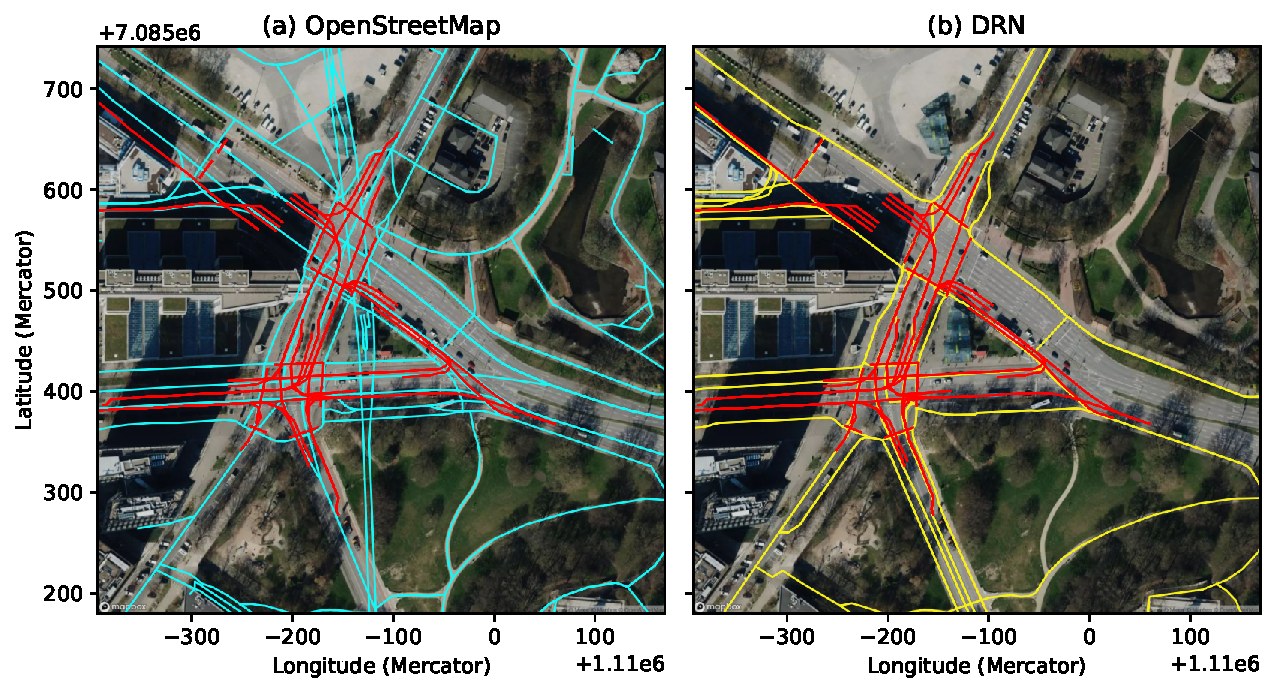
\includegraphics[width=\linewidth]{images/routing-drn-osm-intersection.pdf}
\caption{Alignment of OpenStreetMap vs. DRN with the intersection topology.}
\label{fig:comparison}
\end{figure}

Firstly, the specification in which DRN is presented poses a challenge, requiring a meaningful mapping of DRN's numerous custom path categories to the OpenStreetMap format. Additionally, the geometry of DRN differs from that of OpenStreetMap. Looking at \Cref{fig:comparison} to obtain an initial view of the differences between both datasets, bike paths are usually mapped as separate geometries, generally aligning better with traffic light geometries (denoted in red). However, some secondary paths or roads not intended for cyclists are absent in DRN, requiring additional attention.

An area where the geometric discrepancy becomes problematic is the boundary between both datasets, demarcated by Hamburg's city border. A meaningful connection between the path segments needs to be established to support cross-border routing, even in the presence of imperfect alignments between the path networks. To address this challenge, a stitching procedure will be employed. However, as subsequent sections will reveal, we will face some more routing issues due to the special geometric properties of the DRN dataset. These will also be addressed to obtain a geometrically harmonized hybrid routing foundation. 

Once metadata and geometric structures are harmonized, our final routing foundation will be established. This foundation will enable routing within Hamburg using the DRN dataset and beyond its borders on OpenStreetMap.

\subsubsection{Metadata Harmonization}

\begin{figure}[t]
\centering
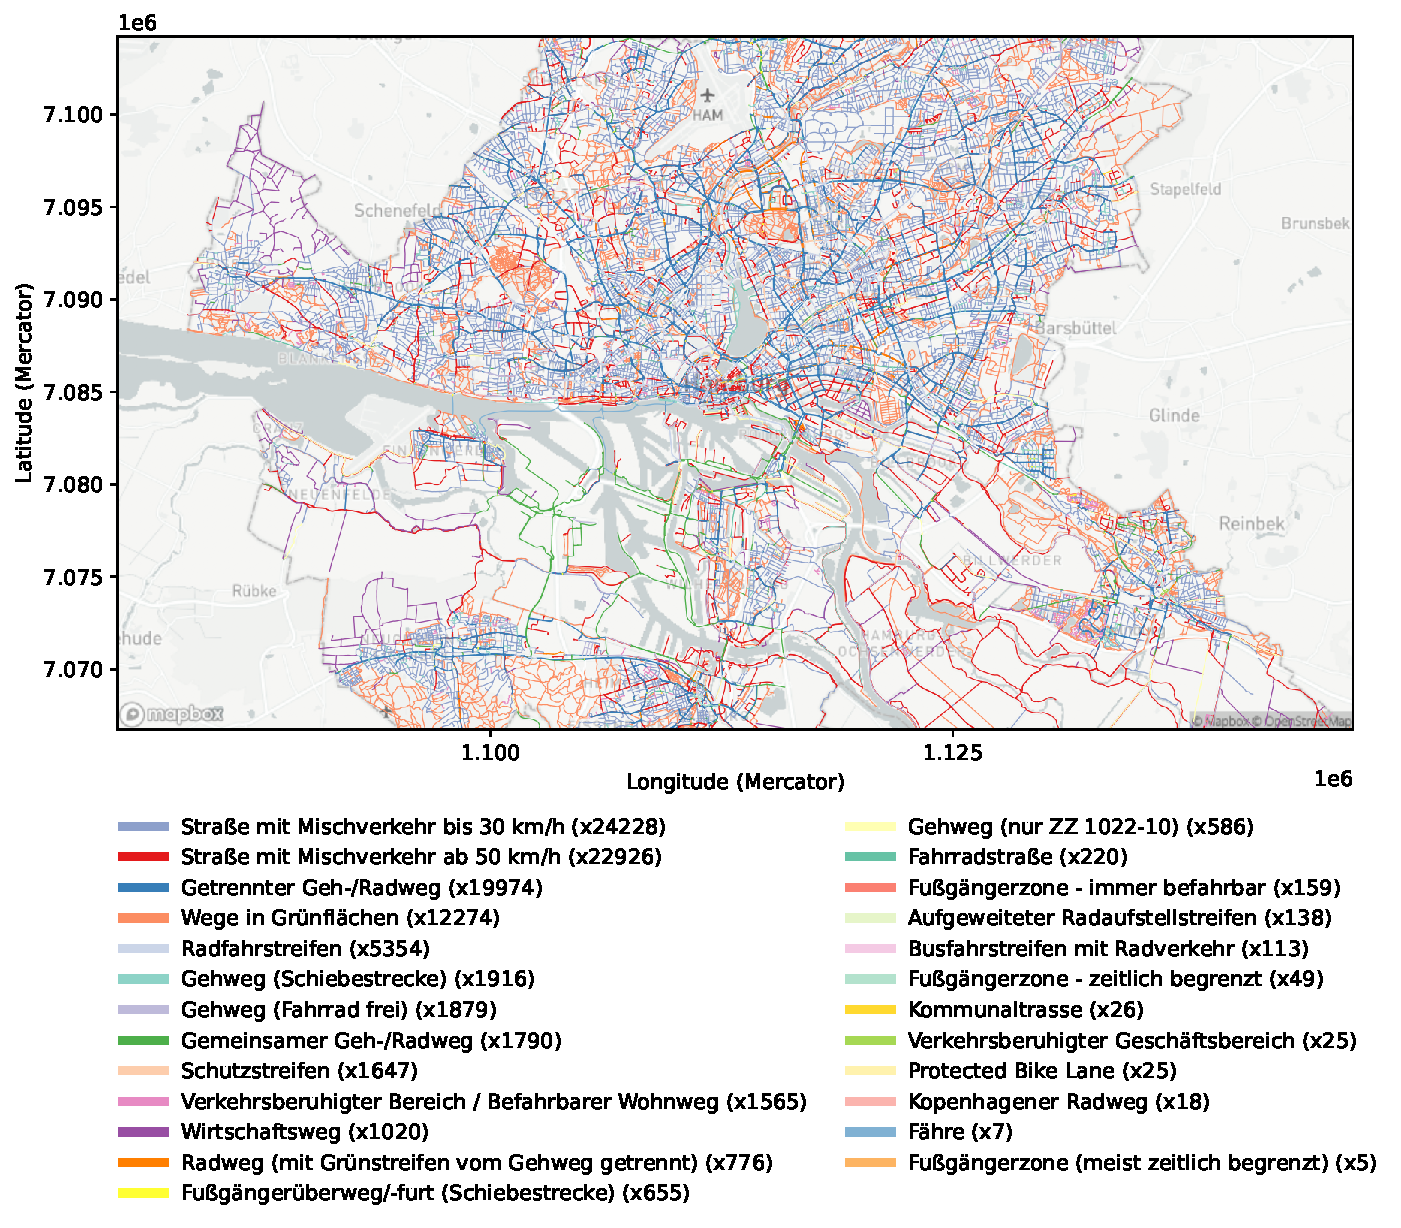
\includegraphics[width=\linewidth]{images/routing-drn.pdf}
\caption{An overview of the DRN dataset and its bike path types, as of Dec 23, 2023.}
\label{fig:drn-map}
\end{figure}

A zoomed-out perspective on the DRN dataset is given in \Cref{fig:drn-map}. The dataset can be downloaded as CSV, GeoJSON, or GML. These formats are typical for geodata but require additional processing to translate them to the specialized \texttt{.osm} format, in which path geometries are given with specific OpenStreetMap attributes. The \texttt{.osm} format allows routing engines to understand bike surface properties and weigh them accordingly through bike-tailored routing profiles.  

Thus, to establish a conversion process from DRN to the \texttt{.osm} format, not only the geometries have to be transformed. Providing the most accurate routing possible requires converting path properties as well. Among others, the following properties are mapped\footnote{The displayed statistics represent a snapshot of the 27th of December 2023.}:

\begin{itemize}
    \item Direction of travel (49813 segments bidirectional and 47606 segments unidirectional)
    \item Time restrictions (32 segments affected)
    \item Temporary paths such as pop-up lanes or detours (83 segments affected)
    \item If a segment is associated with a specific velo route or designated bike tours (Freizeitroute)
    \item Level (96237 flat, 1121 across bridges, 186 through tunnels)
    \item Obstacles (456 impassable, 52 can be circumvented, e.g. via footpath)
    \item The type of bike path and its surface, as illustrated in \Cref{fig:drn-map}
    \item Target and end node ID of the segment connecting the segments to a graph
    \item The segment's coordinates
\end{itemize}

These properties are utilized to infer a corresponding OpenStreetMap class, transforming the DRN dataset into the OpenStreetMap format. This approach of format harmonization lays the foundation for merging both datasets together at the city border. As another benefit, it allows us to reuse existing OpenStreetMap data loaders for routing engines without having to write a custom plugin.

The challenge here is that there is no one-to-one match between all DRN properties and OpenStreetMap properties. For example, DRN specifies three types for compacted surface: "befestigt - nicht genauer erkennbar", "befestigt - zu detailieren" and "Wassergebundene Decke". To resolve this problem, a mapping was developed that assumes the OpenStreetMap tags from the DRN specification. 

The final mapping highlighted in \Cref{tab:tag-mapping} includes the bike path's surface, level, direction, and type. In cases where the bike path's properties cannot be directly mapped to a suitable OpenStreetMap tag, the path is tagged with \texttt{highway=tertiary}. This fallback corresponds to established mapping practices in Germany. The result is an inferred set of tags for each path in the OpenStreetMap format, completing the metadata harmonization process.

\begin{table}[h]
\centering
\caption{Metadata mapping from DRN to OpenStreetMap.}\label{tab:tag-mapping}
\resizebox{\linewidth}{!}{%
\begin{tabular}{p{8.5cm}p{3cm}p{3cm}p{3cm}p{6cm}}
    \hline
    \textbf{Path Type in DRN} & \textbf{\texttt{highway}} & \textbf{\texttt{bicycle}} & \textbf{\texttt{foot}} & \textbf{Other OpenStreetMap Tags} \\
    \hline
    Aufgeweiteter Radaufstellstreifen & \texttt{\textbf{tertiary}} & -- & -- & -- \\
    Busfahrstreifen mit Radverkehr & \texttt{\textbf{service}} & \texttt{\textbf{share\_busway}} & -- & -- \\
    Fähre & -- & \texttt{\textbf{yes}} & -- & \texttt{route=\textbf{ferry}} \\
    Fahrradstraße & \texttt{\textbf{residential}} & \texttt{\textbf{designated}} & -- & \texttt{bicycle\_road=\textbf{yes}, maxspeed=\textbf{30}, source:maxspeed=\textbf{\allowbreak DE:bicycle\_road}, traffic\_sign=\textbf{DE:244.1}} \\
    Fußgängerüberweg/-furt (Schiebestrecke) & \texttt{\textbf{pedestrian}} & -- & -- & -- \\
    Fußgängerzone - immer befahrbar & \texttt{\textbf{pedestrian}} & \texttt{\textbf{yes}} & -- & -- \\
    Fußgängerzone (meist zeitlich begrenzt) & \texttt{\textbf{pedestrian}} & -- & -- & -- \\
    Fußgängerzone - zeitlich begrenzt & \texttt{\textbf{pedestrian}} & -- & -- & -- \\
    Gehweg (Fahrrad frei) & \texttt{\textbf{footway}} & \texttt{\textbf{yes}} & \texttt{\textbf{designated}} & \texttt{traffic\_sign=\textbf{DE:239,1022-10}} \\
    Gehweg (nur ZZ 1022-10) & \texttt{\textbf{footway}} & \texttt{\textbf{yes}} & \texttt{\textbf{designated}} & \texttt{traffic\_sign=\textbf{DE:239,1022-10}} \\
    Gehweg (Schiebestrecke) & \texttt{\textbf{footway}} & -- & -- & -- \\
    Gemeinsamer Geh-/Radweg & \texttt{\textbf{path}} & \texttt{\textbf{designated}} & \texttt{\textbf{designated}} & \texttt{segregated=\textbf{no}} \\
    Getrennter Geh-/Radweg & \texttt{\textbf{path}} & \texttt{\textbf{designated}} & \texttt{\textbf{designated}} & \texttt{segregated=\textbf{yes}} \\
    Kommunaltrasse & \texttt{\textbf{tertiary}} & \texttt{\textbf{share\_busway}} & -- & \texttt{cycleway=\textbf{share\_busway}} \\
    Kopenhagener Radweg & \texttt{\textbf{cycleway}} & \texttt{\textbf{designated}} & -- & -- \\
    Protected Bike Lane & \texttt{\textbf{cycleway}} & \texttt{\textbf{designated}} & -- & -- \\
    Radfahrstreifen & \texttt{\textbf{tertiary}} & -- & -- & \texttt{cycleway:right=\textbf{lane}, cycleway:right:bicycle=\textbf{\allowbreak designated}} \\
    Radweg (mit Grünstreifen vom Gehweg getrennt) & \texttt{\textbf{path}} & \texttt{\textbf{designated}} & \texttt{\textbf{designated}} & \texttt{segregated=\textbf{yes}} \\
    Schutzstreifen & \texttt{\textbf{tertiary}} & -- & -- & \texttt{cycleway:right=\textbf{lane}, cycleway:lane=\textbf{advisory}, cycleway:protection:\allowbreak right=\textbf{dashed\_line}} \\
    Straße mit Mischverkehr ab 50 km/h & \texttt{\textbf{tertiary}} & -- & -- & -- \\
    Straße mit Mischverkehr bis 30 km/h & \texttt{\textbf{residential}} & -- & -- & -- \\
    Verkehrsberuhigter Bereich / Befahrbarer Wohnweg & \texttt{\textbf{living\_street}} & -- & -- & -- \\
    Verkehrsberuhigter Geschäftsbereich & \texttt{\textbf{living\_street}} & -- & -- & -- \\
    Wege in Grünflächen & \texttt{\textbf{path}} & \texttt{\textbf{designated}} & \texttt{\textbf{designated}} & \texttt{segregated=\textbf{no}} \\
    Wirtschaftsweg & \texttt{\textbf{track}} & -- & -- & -- \\
    \hline
    \multicolumn{5}{p{25cm}}{\textbf{Surfaces}: befestigt - nicht genauer erkennbar $\rightarrow$ \texttt{\textbf{compacted}}, befestigt - zu detailieren $\rightarrow$ \texttt{\textbf{compacted}}, Wassergebundene Decke $\rightarrow$ \texttt{\textbf{compacted}}, unbefestigt $\rightarrow$ \texttt{\textbf{unpaved}}, Betonplatten $\rightarrow$ \texttt{\textbf{concrete:plates}}, Bituminöse Decke $\rightarrow$ \texttt{\textbf{asphalt}}, Holz $\rightarrow$ \texttt{\textbf{wood}}, Kunststein-Pflaster $\rightarrow$ \texttt{\textbf{paving\_stones}}, Metall $\rightarrow$ \texttt{\textbf{metal}}, Naturstein-Pflaster $\rightarrow$ \texttt{\textbf{cobblestone}}; \textbf{Obstacles}: Bahnübergang $\rightarrow$ \texttt{\textbf{railway=level\_crossing}}, Treppe $\rightarrow$ \texttt{\textbf{highway=steps}}, Fahrradroute $\rightarrow$ \texttt{\textbf{type=route, route=bicycle, network=lcn}}, Brücke $\rightarrow$ \texttt{\textbf{bridge=yes}}, Tunnel $\rightarrow$ \texttt{\textbf{tunnel=yes}}}. \\
\end{tabular}
}
\end{table}

\subsubsection{Geometric Harmonization}

After the conversion of metadata, the second step is geometric harmonization. However, before we can merge both datasets together, there are still two issues that need further attention: detours resulting from duplicated nodes in the graph and detours because the road cannot be crossed. 

\begin{figure}[ht]
\centering
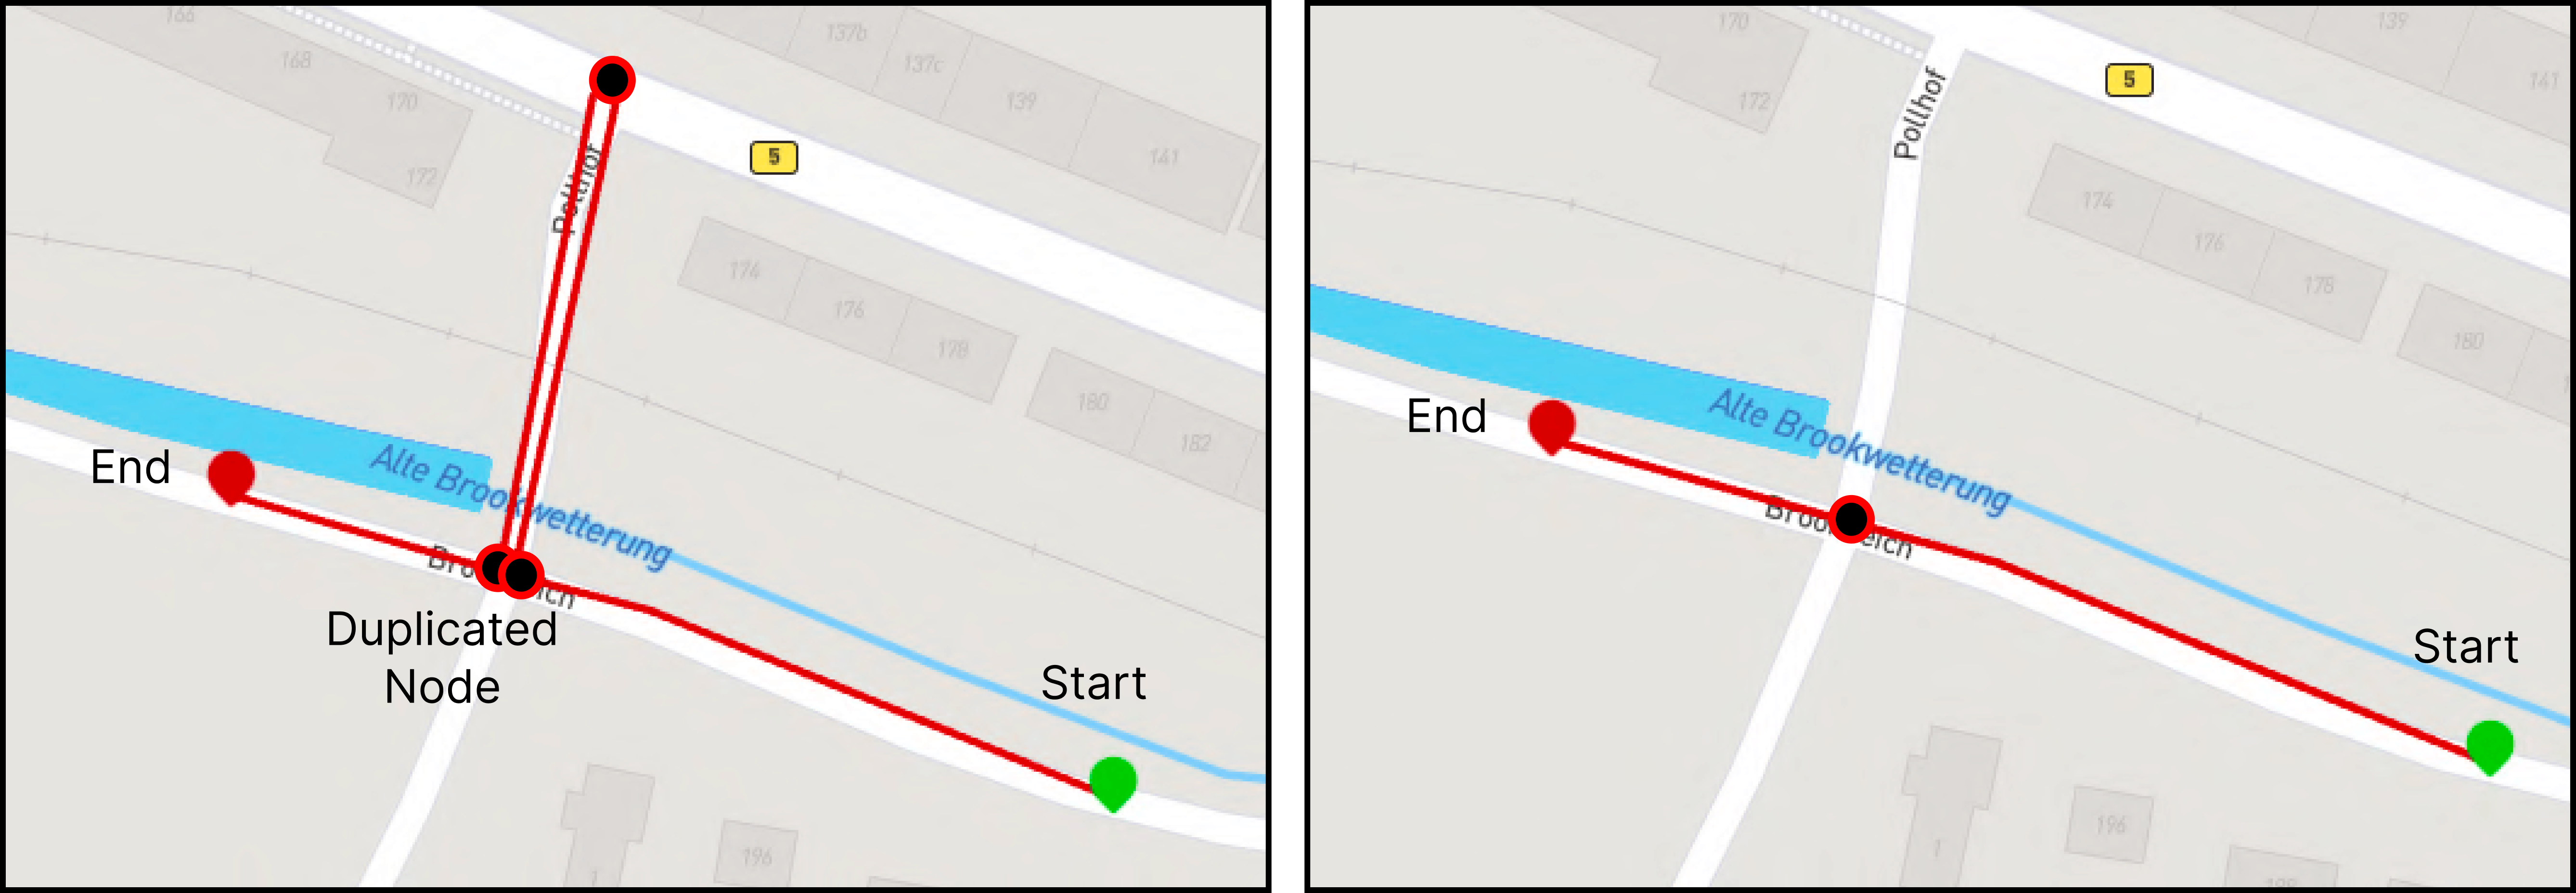
\includegraphics[width=\linewidth]{images/node-merging.png}
\caption{Duplicated nodes (left) are merged together (right) to avoid detours.}
\label{fig:node-merging}
\end{figure}

Each individual path in the DRN dataset starts and ends in a node, which must be transformed into OpenStreetMap nodes that connect the individual paths to a graph structure\footnote{\url{https://wiki.openstreetmap.org/wiki/Node}}. To ease this process, the DRN dataset provides node IDs for the start and end points of each path. Thus, two OpenStreetMap nodes need to be generated for each DRN path based on the start and end coordinates given in the line geometry. 

Since there may be multiple DRN paths that are connected to a single OpenStreetMap node, the same node is generated multiple times during dataset processing. In theory, this should not be a problem since the node ID can be utilized to avoid duplicates. In practice, however, sometimes there are nodes for which multiple different coordinates are found in the dataset, presumably due to floating point inaccuracies of a preceding geographic projection step during dataset publishing. As highlighted in \Cref{fig:node-merging}, this leads to the issue of duplicated OpenStreetMap nodes in the proximity of a few centimeters that are not properly connected.

The developed solution involves merging all found coordinates for a specific node ID into a center point. Let $C_k = \{c_{k_1} = (lat_{k_1}, lng_{k_1}), \text{...} , c_{k_n} = (lat_{k_n}, lng_{k_n})\}$ be the collected coordinates for each node $k$. Then, the center point $\text{Center}_{\text{k}}$ is calculated as the mean of all coordinates for that node ID:

\begin{equation}\text{Center}_{\text{k}} = \left(\frac{\sum_{i=1}^{|C_k|} \text{{lat}}_{k_i}}{|C_k|}, \frac{\sum_{i=1}^{|C_k|} \text{{lng}}_{k_i}}{|C_k|}\right)\end{equation}

This method assumes small distances between the coordinates that are not noticeably affected by the curved WGS84 projection system. The maximum relocation distance between all $\text{Center}_{\text{k}}$ and $c \in C_k$ was calculated as 8.3 centimeters using the haversine formula. Based on this preliminary validation, no further points are falsely connected. Thus, this first issue could be resolved without any further challenges and without manual processing.

The second issue in the DRN dataset requiring additional processing is non-crossable roads, as highlighted in \Cref{fig:oneway-travel-fix}. Since bike paths on both roadsides are captured as individual geometries in the DRN dataset, there may be long road segments with bike paths running in parallel. However, without interconnections between the roadsides, there is also no possibility for the route to cross the road. Sometimes, this represents a problem since side roads attached to the opposite roadside can only be reached by long detours. With OpenStreetMap, this is a lesser problem since roads are often captured as single-path geometries without a clear distinction between each roadside. 

\begin{figure}[htbp]
\centering
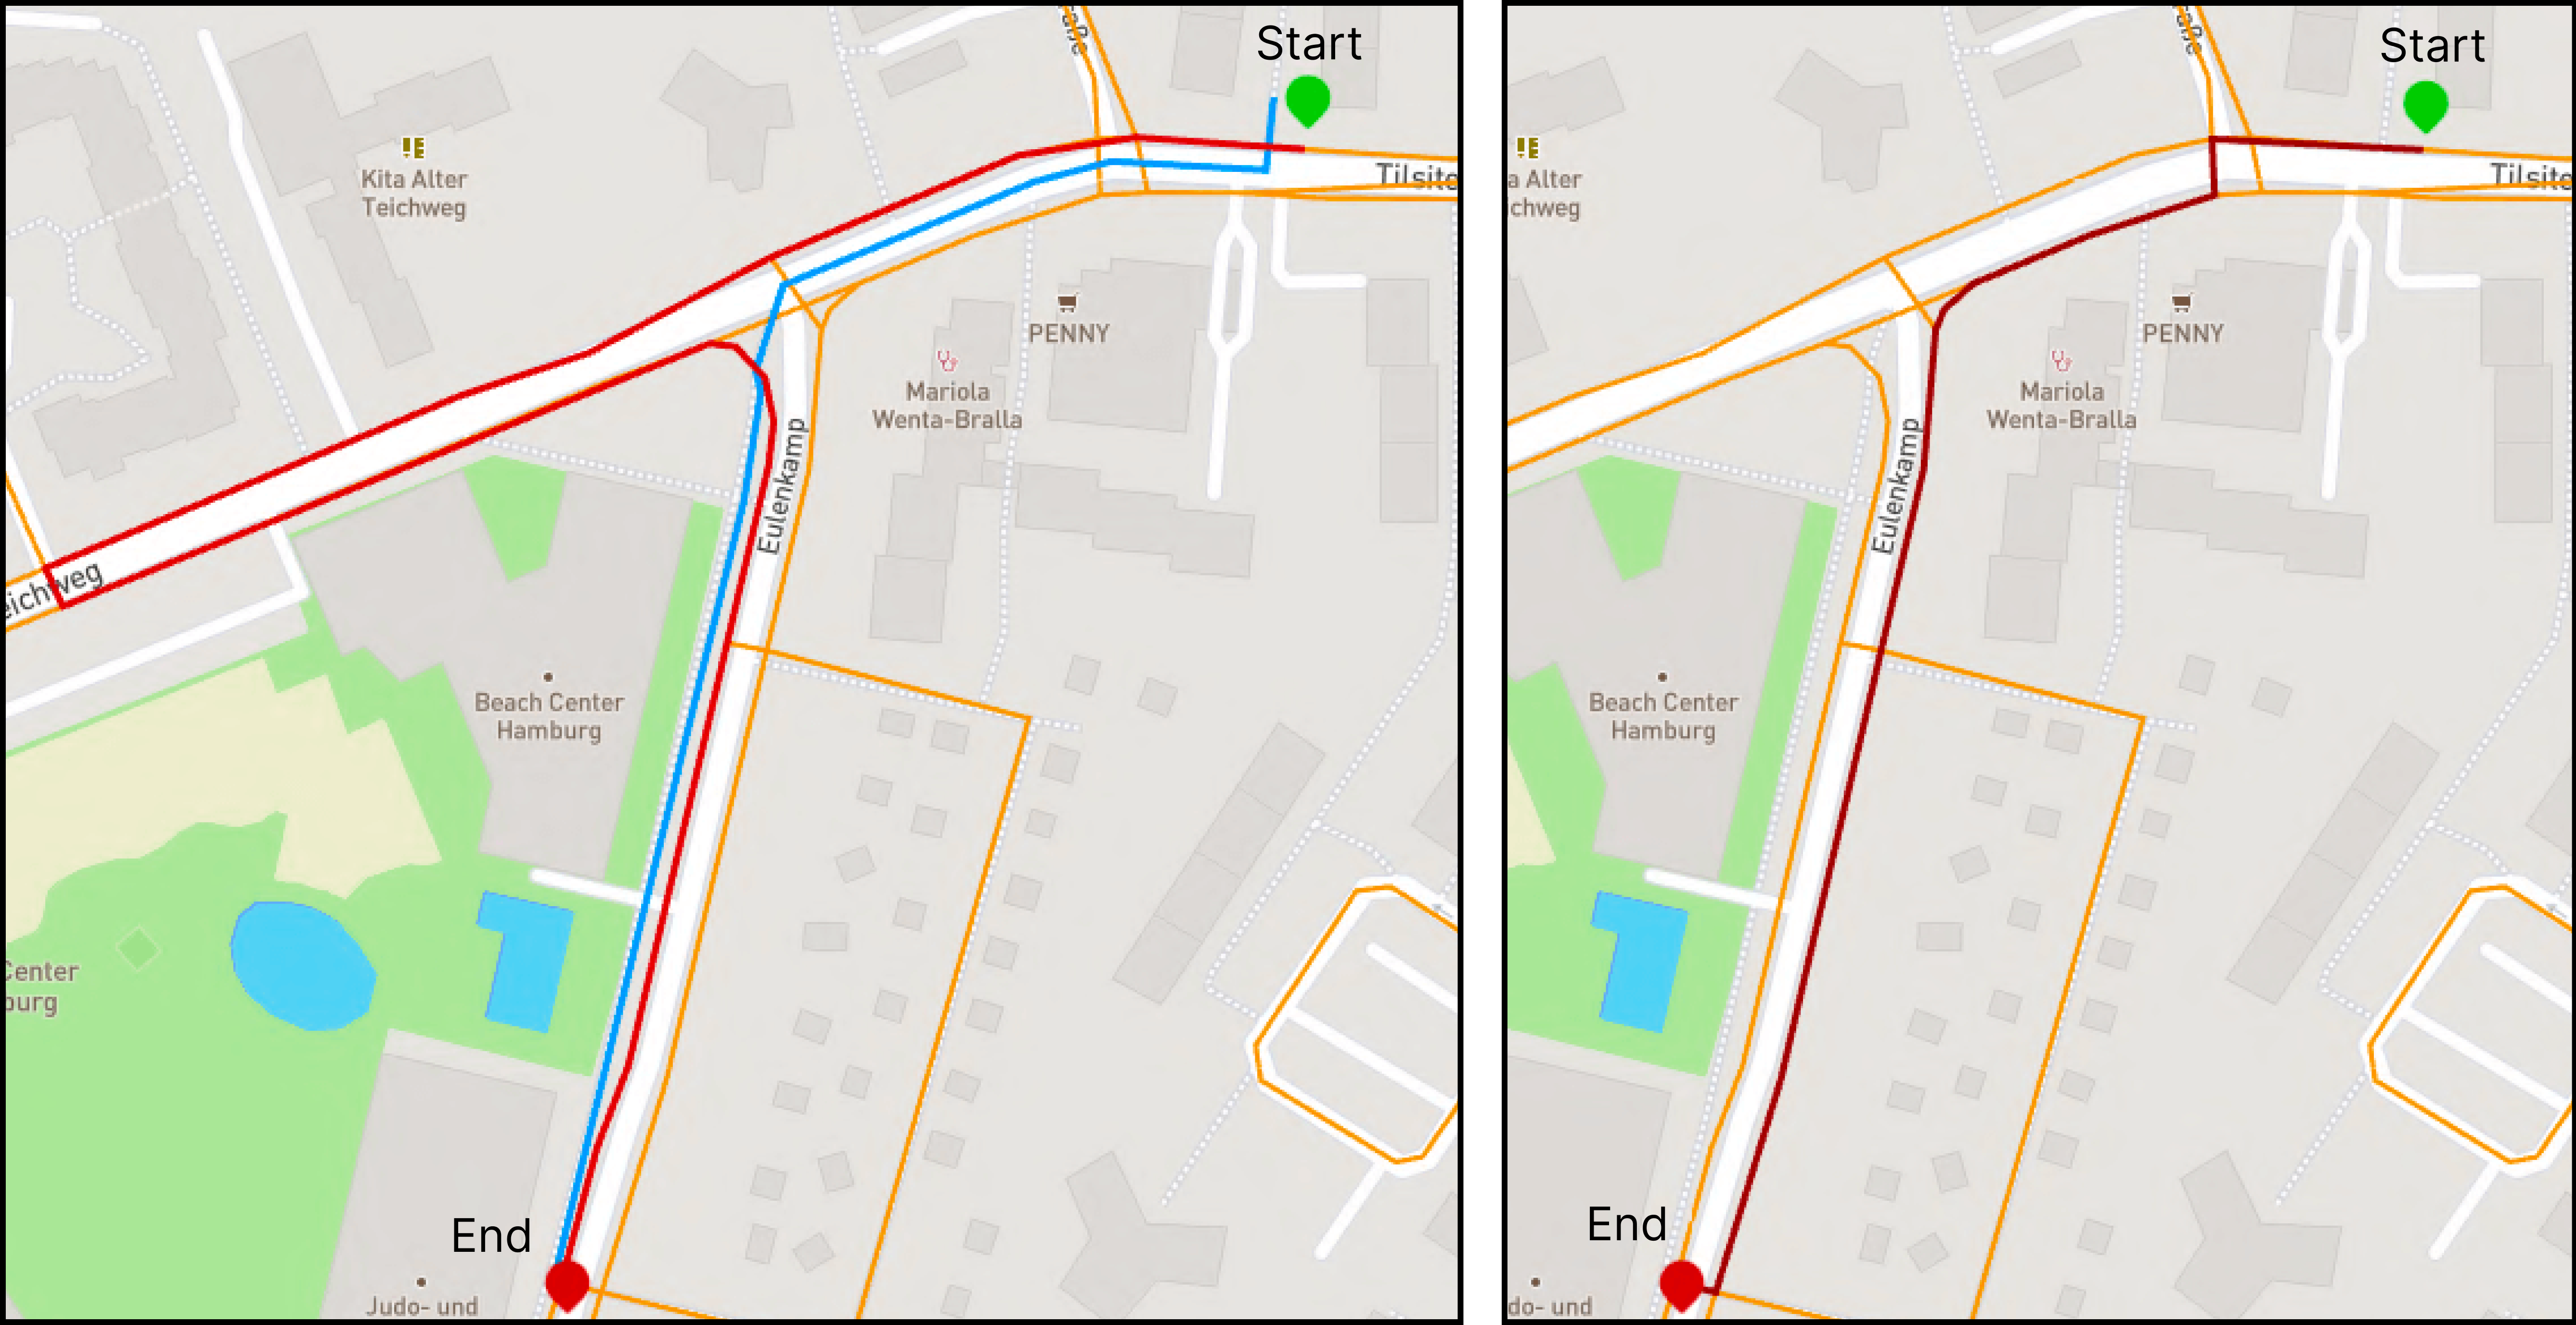
\includegraphics[width=\linewidth]{images/oneway-travel-fix.png}
\caption{Detour (left) that can be fixed by enabling opposite-direction one-way travel on foot (right), compared to OpenStreetMap route (blue).}
\label{fig:oneway-travel-fix}
\end{figure}

One explored solution is the introduction of "virtual" paths connecting the roadsides. Using these paths, the route could traverse between roadsides and avoid detours. Although this concept may sound like a reasonable idea at first, the question is where to place these virtual paths. For example, one could place these paths in a fixed interval along a road between roadsides. However, there could always be a physical barrier between both roadsides, meaning that generated routes would guide users over impassable obstacles or potentially encourage dangerous maneuvers. Traversing a road at an arbitrary location may not always be safe or legal. Due to these reasons, the idea of inserting virtual paths was discarded.

The final solution takes another approach. In the DRN dataset, bike paths are marked for travel in one direction or two directions. Here, the error source for detours is often the restricted one-way travel direction along the bike path. In cases where detours are observed due to long paths down the street until the next road crossing, it is likely that a similar road crossing lies closer up the street. Thus, a solution is to allow opposite-direction one-way travel on foot. This solution assumes that the bike can safely and legally be dismounted and walked in the opposite direction.

Having addressed the issues of duplicated nodes and detours due to non-crossable roads, no further issues have presented themselves. Thus, we can now focus on the merging of both datasets along the city border. The conflation process starts with matching the OpenStreetMap paths to the associated DRN paths along the city border. First, DRN nodes close (<20m) to the border are fetched. For each of these DRN nodes, the five nearest OpenStreetMap paths are treated as a possible match. 

\begin{figure}[t]
\centering
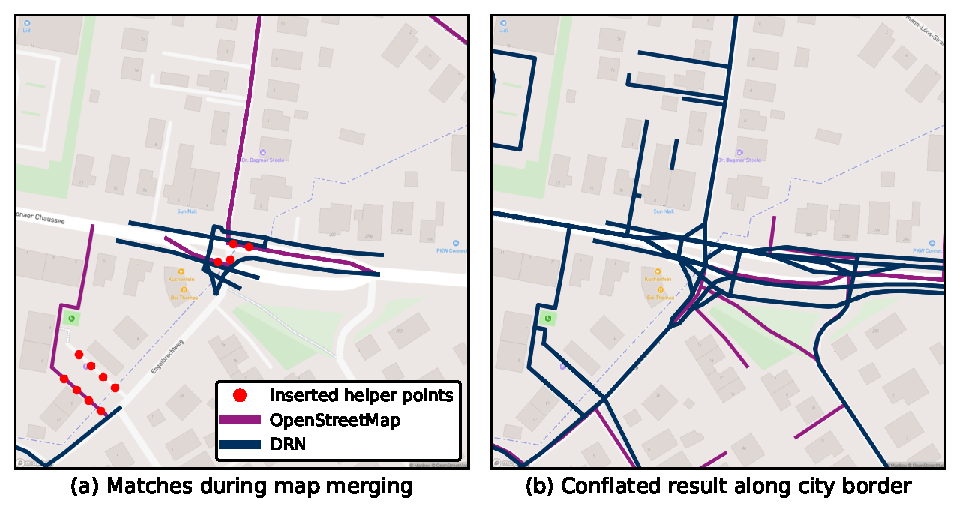
\includegraphics[width=\linewidth]{images/routing-drn-osm-border.pdf}
\caption{.}
\label{fig:routing-drn-osm-border}
\end{figure}

However, the OpenStreetMap paths may traverse the city border without a node lying exactly on the border geometry, potentially leading to z-shaped connections between OpenStreetMap and DRN. To avoid this problem, the conflation process inserts artificial OpenStreetMap nodes at the intersection of the city border geometry. These additional nodes are illustrated in \Cref{fig:routing-drn-osm-border} as helper points. Finally, for each DRN node, the nearest interpolated OpenStreetMap node is selected and connected. This process is highlighted in \Cref{fig:routing-drn-osm-border}, transitioning the DRN network over its original boundary into OpenStreetMap geometries, which can be clearly seen in the example.

After the geometric harmonization is finished and all DRN path tags are converted into the OpenStreetMap format, the path network is exported in the \texttt{.osm} format. This step finishes the overall merging process, delivering a map file that can be loaded by any routing engine that supports the OpenStreetMap format. All described steps are performed fully automatically in a single processing pipeline, allowing daily updates to the routing foundation without human intervention in the merging process. This allows changes to the cycling infrastructure to be reflected timely in the routing service, assuming the dataset provider updates DRN on a regular basis. 

Additional changes resulting from quality assurance to the existing paths are also automatically imported. During the process of testing the DRN routing, four issues with missing path geometries in the path network were encountered and reported via an e-mail address described on the dataset download page, leading to correction and response within one day by the dataset maintainers. Two additional geometries we initially interpreted as missing based on satellite images were apparently correct due to ongoing construction on site. Thus, if issues are encountered during usage of the integrated network, the quality assurance process can be considered timely overall, while proposed changes appear to be cross-checked.

\subsection{Integration}

So far, we have investigated how to establish a routing foundation based on the DRN dataset. However, the routing foundation itself is only one part of delivering accurate bike routes to users. Integrating this routing foundation as a service into the bike-GLOSA application requires a few additional steps. First, the routing foundation must be incorporated into a routing engine and deployed in a backend service. Afterward, specific routing profiles must be selected that enable personalized bike routing. Leveraging the inclination sensitivity of bike routing profiles necessitates selecting a suitable height provider. Finally, the routing can be applied inside the mobile application for distance-to-signal estimation and GNSS error correction. The end of this section discusses the employed rerouting strategy to ensure that users can still properly reach their destination even when deviating from the originally planned route.

\subsubsection{Automated Deployment}

\begin{figure}[ht]
\centering
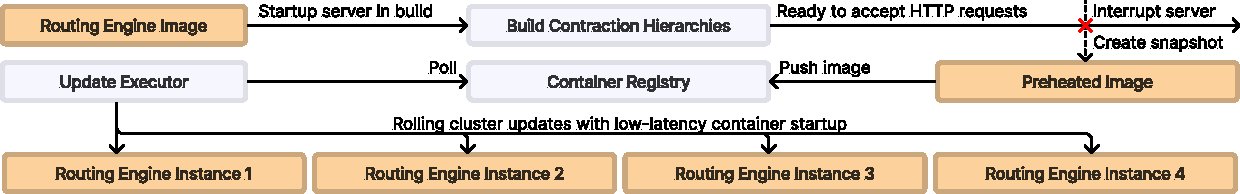
\includegraphics[width=\linewidth]{images/load-distribution-containerization-preheating.pdf}
\caption{CI/CD pipeline for automated rollouts of routing network updates.}
\label{fig:multi-stage-continuous-deployment}
\end{figure}

As a routing engine, we will choose the state-of-the-art solution GraphHopper that we have referenced in the related work section. GraphHopper is not only open source, it also provides access to community-tested bike routing profiles that we will reuse for route personalization. In addition, GraphHopper is also compatible with various height data providers and implements inclination-sensitive routing profiles. 

Using the \texttt{.osm} format, we can simply configure GraphHopper to load our DRN routing. Then, the GraphHopper service is packaged together with the DRN routing data into a Docker image and deployed on our Docker Swarm backend. Through the pipeline highlighted in \Cref{fig:multi-stage-continuous-deployment}, we configure a nightly build of the Docker image, including fetching and merging the current DRN data. An update executor on the orchestrator machine notices the updated Docker image and replaces the currently deployed service using a rolling update, ensuring that the running services always work with the newest map materials. 

Since GraphHopper requires time to preprocess the routing network on the first startup, the container startup is not immediate after it is rolled out to one of the replicated worker machines. Thus, allowing direct access to the starting routing engine could result in requests from clients failing. Two measures are employed to circumvent this issue. First, Traefik\footnote{\url{https://traefik.io/traefik/}} is utilized as a frontline proxy for the Docker Swarm and configured to direct only requests to healthy containers. A health check is implemented on the routing Docker container, allowing requests only once the container is started up. Additionally, to further accelerate the startup of each routing service container, the Docker image is preheated. Starting up GraphHopper during the build process and waiting for its routing API to become available makes the routing engine available faster after rollout. 

\subsubsection{Inclination-Sensitive and Personalizable Routing}

When deployed, GraphHopper provides different \texttt{vehicle}s with individual path weights depending on the road's properties. Each \texttt{vehicle} represents a different routing profile. Among these \texttt{vehicle}s are also various bike types such as \texttt{bike}, \texttt{bike2} (avoids inclines), \texttt{racingbike} or \texttt{mountainbike}. These profiles can be provided to the routing API to select a specific behavior, such as avoiding unpaved sections with the \texttt{racingbike} profile. However, one challenge is selecting the best routing configuration for a user's needs. 

Initially, the idea existed to infer the best routing profile, or even a custom routing profile, based on the user's recorded trajectories. However, this idea was discarded in favor of a much simpler and more robust approach, avoiding the danger of overemphasizing user data and providing inconsistent routes between multiple devices with the same configuration. Instead, users are given a menu as depicted in \Cref{fig:routing-profile-mapping} providing three options: bike type, route preference (fast, comfortable), and whether inclines should be avoided. Using these selections, a suitable routing profile is mapped. This allows two users to share and ride the same route together without any further issues.

Here, it should be noted that a short routing option was also provided preliminarily, in addition to fast and comfortable routing. However, routes generated with this routing profile would frequently lead over the wrong roadside since both roadsides are captured independently in DRN. The ported DRN network is configured with walking speeds in the opposite allowed direction, assuming users have to dismount their bicycles to correspond to road laws. As a result, another issue with routing on the opposite roadside was that travel times were increased significantly, reported as a bug by test users. Hence, the short routing profile was excluded from the available options. The other routing profiles do not have this problem since they also consider the travel time that is significantly increased traveling in the opposite direction.

\begin{figure}[t]
\centering
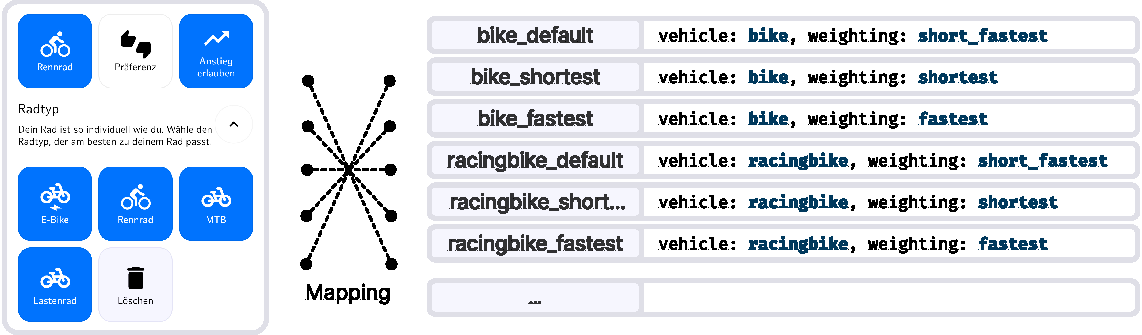
\includegraphics[width=\linewidth]{images/routing-profile-mapping.pdf}
\caption{Mapping of routing profiles for route personalization.}
\label{fig:routing-profile-mapping}
\end{figure}

In case users don't specify a routing profile, a default routing profile (\texttt{bike2}) is selected that utilizes the \texttt{short\_fastest} weighting, which represents a compromise between the short and fast weightings. This routing profile also tends to avoid inclines, incorporating height data into the route-finding process.

In Hamburg, inclinations may be less of a concern, but there are still several roads with non-negligible inclines, such as Helgoländer Allee. To supplement the routing engine with the necessary height data that is not provided by DRN (or OpenStreetMap), there are multiple digital elevation models that can be used. By default, GraphHopper supports SRTM (Shuttle Radar Topography Mission) \cite{farr_shuttle_2000, farr_shuttle_2007} and CGIAR \cite{jarvis_hole_2008} height data. The CGIAR height data is a proprietary post-processed version of the SRTM data, filling in data gaps in the SRTM height map, and is available under license to all GraphHopper users. By default, the routing engine is specified to use the SRTM dataset.

SRTM-1 offers a horizontal resolution of approximately 30m (1 arcsecond). For specific areas, additional SRTM X-SAR 25m data is provided by the DLR. For the covered regions of the SRTM X-SAR 25m model, the vertical precision is specified at $\pm$ 6m (relative vertical error at 90\% confidence level)\footnote{SRTM X-SAR 25m specification: \url{https://geoservice.dlr.de/web/dataguide/srtm/}}. An even higher precision is offered by the DGM-1 model for Hamburg, in which the one stands for one meter of horizontal resolution. In DGM-1, the vertical resolution is specified as $\pm$ 15cm\footnote{\url{https://metaver.de/trefferanzeige?docuuid=A39B4E86-15E2-4BF7-BA82-66F9913D5640}}. The high precision is reached by airborne laser scanning. Downscaled resolutions are available as DGM-10 (10m) and DGM-25 (25m).

To evaluate if the DGM models provide an overall better height profile than SRTM, cross-sections of the height models were analyzed by Max Lorenz. Another important question was how much resources the model consumes when loaded into the routing engine. The results indicated that the best tradeoff between resource usage and model accuracy is provided by the DGM-10 model. Thus, the DGM-10 model was integrated as the final digital elevation model into the GraphHopper routing engine using a custom tileset download and parsing plugin. The result is a GraphHopper routing engine that not only runs on the DRN dataset but also utilizes the DGM-10 model to provide accurate, personalized routing while consuming an acceptable amount of resources. 

\subsubsection{Distance-to-Signal Estimation and Mitigating GNSS Inaccuracies}

Focusing further on the applications of the developed routing engine within our GLOSA application, a distance estimation method was designed that aims to be more accurate than just taking the direct (linear) distance to the user's position. This method assumes that the route closely aligns with the actual bike infrastructure, ensuring an accurate estimation.

\begin{figure}[t]
\centering
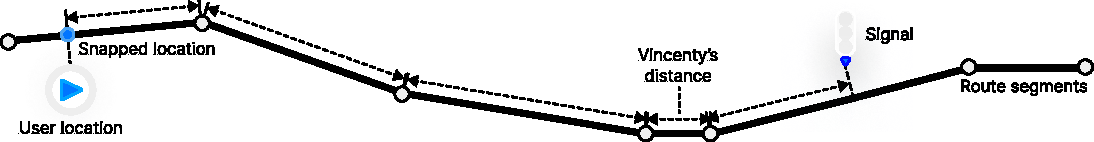
\includegraphics[width=\linewidth]{images/distance-to-signal-estimation.pdf}
\caption{Distance-to-signal estimation along the route curvature for speed recommendation.}
\label{fig:distance-to-signal-estimation}
\end{figure}

The specific process is highlighted in \Cref{fig:distance-to-signal-estimation}. First, the user's location is snapped to the route geometry, and the subsequent route segments are traversed until reaching the snapped location of the upcoming traffic light. The locations of each traffic light are annotated to the route geometry using the traffic light matching method developed in \Cref{ch:matching}.

Along the precalculated route segments, the distance is determined using the Vincenty estimator, which provides a more accurate distance measure (up to 0.5mm) than the haversine distance through a more accurate representation of the earth's shape while being slightly more computationally expensive. To further optimize the computational overhead, the distances to each traffic light are precalculated along each route segment. With this approach, it is only necessary to calculate the distance along the current segment and then add this segment's distance to the next traffic light. The distance estimation process is repeated dynamically each time a new user location is received, updating the current speed advisory.

A second application of the route geometry within the app is for GNSS error correction, which arose not only as one of the major challenges for GLOSA applications in related work but also during preliminary experiments of the mobile app. Tests conducted in Dresden indicated that older devices (Android 6) struggle more with GNSS drift than newer devices. Even the latest generation of Android and iOS smartphones, configured to provide the highest level of geolocation accuracy, seem to experience this problem.

Assuming that the user strictly follows a predefined route, we can simply snap the user's location to the route, eliminating any GNSS scattering orthogonal to the route. GNSS scattering in the direction of the route is not eliminated. Thus, route snapping alone has the drawback that, when approaching a traffic light slowly, the measured location may jump beyond the traffic light with respect to the route. 

To mitigate this problem, GNSS drift at an intersection is detected as follows: if the user is moving at a GNSS speed less than 2 meters per second, the app reverts to the last traffic light if it is within 10 meters of the user and no other traffic light is closer. In case a traffic light is still overshot, the user also has the option to manually switch between traffic lights through the application's user interface. In case a user fully deviates from the designated route, automated rerouting is performed. Here, it is important to avoid triggering rerouting for minor GNSS errors when the user is still following the route accurately.

\subsubsection{Automated Rerouting}

\begin{figure}[t]
\centering
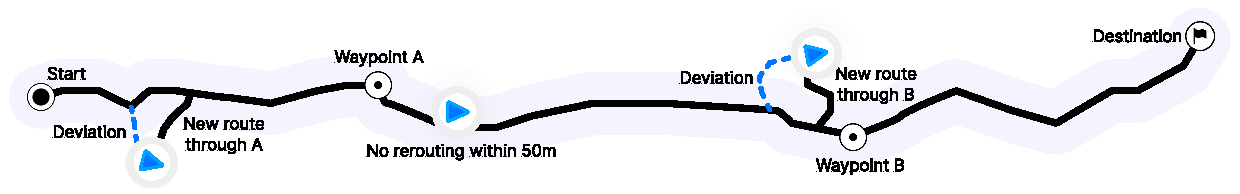
\includegraphics[width=\linewidth]{images/rerouting-strategy.pdf}
\caption{Schema of the rerouting procedure using a triggering threshold of 50 meters from the route.}
\label{fig:rerouting-strategy}
\end{figure}

The developed rerouting approach operates as illustrated in \Cref{fig:rerouting-strategy}: while the user is on the move, their location is continuously compared to the route by aligning it with the route geometry. The distance between the aligned location and the actual location is measured against a threshold. When the user moves significantly away from the route, exceeding the threshold, the rerouting is automatically initiated. 

A challenge in this approach is determining the appropriate distance threshold that strikes a balance between prompt rerouting and avoiding unnecessary recalculations. In initial tests conducted in Hamburg, a threshold of 20 meters was used. However, it proved to be too low and resulted in excessive unnecessary reroutings during field tests. Consequently, the threshold was increased to 50 meters, which yielded a satisfactory balance.

\begin{figure}[t]
\centering
\resizebox{\linewidth}{!}{%
\begin{tabular}{p{0.5\linewidth}p{0.5\linewidth}}
  \multicolumn{1}{c}{\small{(a) Rerouting via closest waypoint.}} &
  \multicolumn{1}{c}{\small{(b) Rerouting via virtual waypoint connection.}} \\
  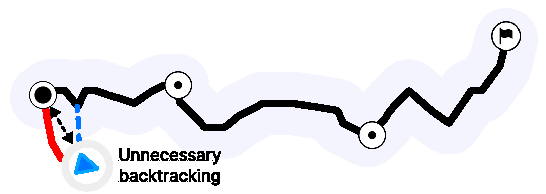
\includegraphics[width=\linewidth]{images/rerouting-strategy-1.pdf} &
  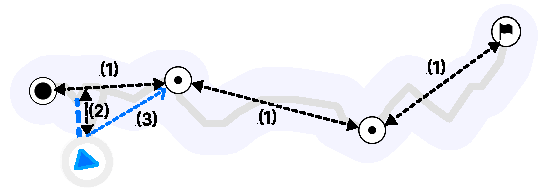
\includegraphics[width=\linewidth]{images/rerouting-strategy-2.pdf}  \\
\end{tabular}
}
\caption{Schematic comparison of the initial and final rerouting algorithms.}
\label{fig:rerouting-strategy-comparison}
\end{figure}

An additional challenge in this approach is identifying the waypoints that have already been visited to prevent rerouting back to the starting point. To address this issue, only the remaining waypoints are selected when rerouting is triggered. Originally, the rerouting process involved selecting the nearest waypoint to the user and recalculating the route using that waypoint as a reference. However, this method depicted in \Cref{fig:rerouting-strategy-comparison} on the left was only effective half of the time, assuming the user's location was closer to the upcoming waypoint than to the previously visited waypoint. Consequently, this initial strategy often led to unnecessary backtracking.

Another option considered was snapping the user's location to the route geometry and following that path to find the next waypoint. However, a challenge arose because the waypoints were not directly integrated into the route geometry data structure, which is returned from the routing framework. Although it is possible to align the waypoints with the route geometry for implementation, a simpler and faster approximation was employed in the app, consisting of three steps: (1) Drawing direct lines between waypoints to create a connected path roughly resembling the route. (2) Selecting the nearest line to the user's location. (3) Determining the waypoint at the end of this line as the next waypoint for recalculating the route. This approach assumes that the drawn lines approximately represent the general route structure.

\begin{Summary}[Summary of Methods]
To provide accurate bike routing in Hamburg, we investigate the usage of an authoritative dataset for bike infrastructure, DRN. Preparing the DRN dataset for routing, we first translate the path descriptions given in the DRN dataset into the OpenStreetMap format. This allows our routing engine to assign different costs to each path segment depending on its properties, circumventing uncomfortable paths for more sensitive bike types such as racing bikes. Afterward, we address two specific kinds of issues that were detected in the DRN dataset. Duplicated and slightly misaligned nodes are combined using their center point, and the opposite direction of every path is marked passable if on foot. As a result, routes no longer take long detours to cross a road in case a much closer crossing is available upstream. Finally, we stitch the boundary region of DRN using helper points to allow cross-border routing between OpenStreetMap and DRN. 

The fully automated processing pipeline is utilized by the deployment infrastructure to roll out new map material on a daily basis. Preheating of the routing engine is employed to accelerate service rollouts. Inclination- and person-sensitive routing is implemented through a menu that allows users to configure their desired options and realized through the DGM-10 height provider that provides the best resource-accuracy tradeoff. The distance to the next traffic light is extrapolated through the route segments on which the traffic lights and their distances along the route are annotated. Snapping the GNSS position to the next route segment updates the speed advisory through the newly calculated traffic light distance but also eliminates GNSS scattering orthogonal to the route. GNSS scattering along the route is mitigated by detecting situations in which the position erroneously jumps over a traffic light before which the user is standing. A rerouting is initiated after the user deviates more than 50 meters from the route, selecting the remaining waypoints without inducing unnecessary backtracking to already passed ones. 
\end{Summary}

\section{Results}

Whether the goal of a more accurate bike routing could be reached will be evaluated in four steps. First, we will investigate the general structure of the processed routing network and compare its completeness to OpenStreetMap. Specifically, we will focus on the path categories that were mapped using our metadata mapping from the DRN format and compare these to the OpenStreetMap network. 

Afterward, a ground truth -- hand-drawn reference tracks -- will help us evaluate how well DRN routes align with actual cycling infrastructure. Here, we will also compare DRN with Google Maps and Bing Maps. Analyzing an arbitrary sample of DRN routes, we will investigate how many routing errors are encountered.

In the third part of our evaluation, we will revisit the traffic light matching results from \Cref{ch:matching}, retrain our matching models on a new ground truth, and investigate whether the accuracy can be improved. Studying the alignment between traffic light geometries and DRN routes, we further investigate the change in traffic light matching accuracy. In a more coarse-grained study, we also capture routing errors at intersections to find whether the problem of routing on the road instead of bike paths could be resolved. 

After we have compared the routing accuracy to a hand-drawn ground truth and traffic light geometries, we validate our results with our users' recorded GNSS trajectories. In this study, we also compare our approach to distance-to-signal estimation with the linear distance approach to find in which situations our approach may perform better or worse. Finally, we will investigate where and how often users deviate from precalculated routes, together with its relationship to the preselected routing profile.

\subsection{Completeness}

\begin{figure}[t]
\centering
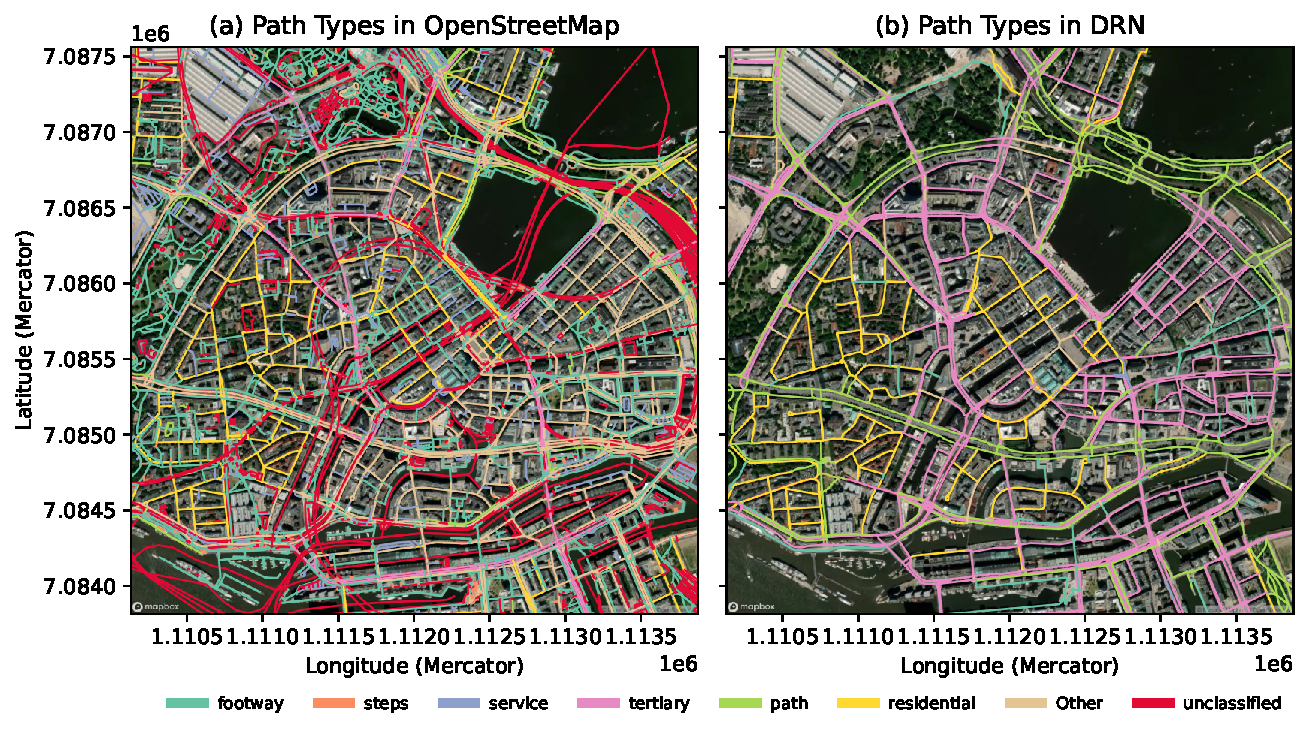
\includegraphics[width=\linewidth]{images/routing-drn-osm-map.pdf}
\caption{Mapping of path types.}
\label{fig:routing-drn-osm-map}
\end{figure}

Based on an analysis conducted by Max Lorenz, the converted DRN path network encompasses roughly 7,689 kilometers in comparison to OpenStreetMap, which covers approximately 10,557 kilometers. The reported coverage for OpenStreetMap excludes paths inaccessible for cyclists, marked with \texttt{highway=motorway}, \texttt{highway=motorway\_line}, \texttt{highway=trunk\_link}, \texttt{access=private}, or \texttt{bi\allowbreak cycle=no}. Footpaths are also excluded unless bicycles are allowed with \texttt{bicycle=yes}. 

The size difference is mainly due to additional accessory paths that are contained in OpenStreetMap but not on DRN. As a consequence, when generating 10,000 random routes throughout the city, the average distance that has to be traveled to the next available path segment varies slightly: 77.04 meters in DRN and 52.80 meters in OpenStreetMap. Even though the DRN network seems to encompass fewer paths, those that are captured are more detailed. The average path segment length in OpenStreetMap was calculated as 102.39 meters compared to 79.16 meters in DRN.

The structural differences are highlighted in \Cref{fig:routing-drn-osm-map}. Here, it can not only be seen that OpenStreetMap provides more accessory paths, but also its higher diversity in path categories than present in the mapped DRN network. It can also be seen that DRN tends not to capture ways through green spaces. As a result, one minor drawback is that routes with DRN can be generated until the border of a park area but not inside or throughout. The same is true for intermodal connections such as railroads and ferries, which are mapped as unclassified paths in the displayed example. DRN does not capture these connections.

\begin{figure}[t]
\centering
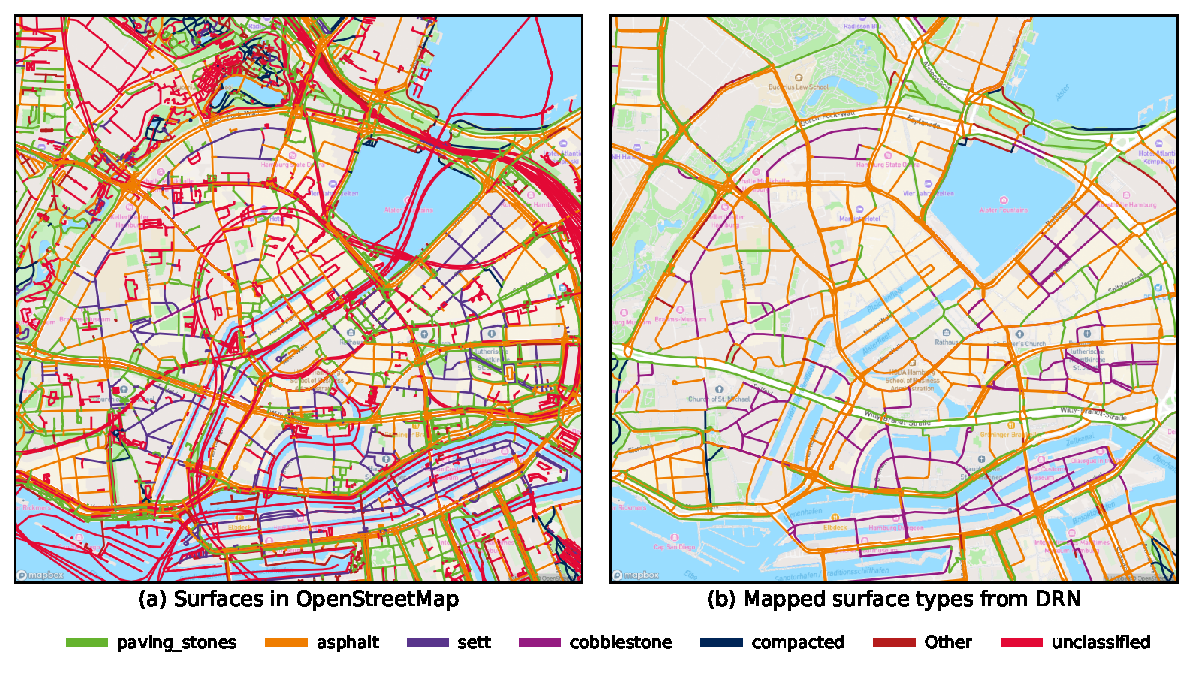
\includegraphics[width=\linewidth]{images/routing-drn-osm-map-surfaces.pdf} 
\caption{Mapping of surface types.}
\label{fig:routing-drn-osm-map-surfaces}
\end{figure}

On the other hand, as seen in \Cref{fig:routing-drn-osm-map-surfaces}, OpenStreetMap contains large proportions of paths with an unclassified surface. Overall, only 66.4\% (7,014.52 km) of paths in OpenStreetMap's representation of Hamburg are tagged with a surface, as opposed to 99.9\% (7,682.24 km) in the DRN network. However, OpenStreetMap also contains an additional surface quality tag for 783.56 km (7.4\%), which is not mapped by our approach but can be parsed by GraphHopper as an additional source of information to estimate the path speed\footnote{\url{https://github.com/graphhopper/graphhopper/blob/71d2de049f2f4f52453a6fb1b7d558b9f0fa011f/core/src/main/java/com/graphhopper/routing/util/parsers/BikeCommonAverageSpeedParser.java\#L103}}. 

Other metadata, such as road width, is even rarer in OpenStreetMap, with only 9.2\% (704.47 km) of paths containing this information, in contrast to 99.9\% (7,687.69 km) in the DRN routing foundation. An additional property analyzed is the coverage of velo routes, which resides at 1,794.55 km in OpenStreetMap and 1,149.8 km in DRN.

Overall, despite fewer paths being captured, the DRN network offers more detailed and well documented path segments, with a higher percentage tagged with surface information, road width, and other valuable metadata. As it is the goal of DRN to capture bike paths accurately to their actual position, it is generally not a problem if intermodal connections are not contained. However, a higher coverage of green spaces and accessory paths could be desirable. 

\subsection{Alignment with Actual Bike Paths}

To measure the alignment of generated bike routes with actual cycling infrastructure, we create a separate ground truth by hand-drawing reference bike paths with the help of satellite imagery. Although we will not reach centimeter-level accuracy with this method, it will help measure general misalignments in the bike routes that we have encountered previously. This method generally assumes quite recent satellite image tiles that are aligned well with the actual position using an appropriate projection.

\begin{figure}[t]
\centering 
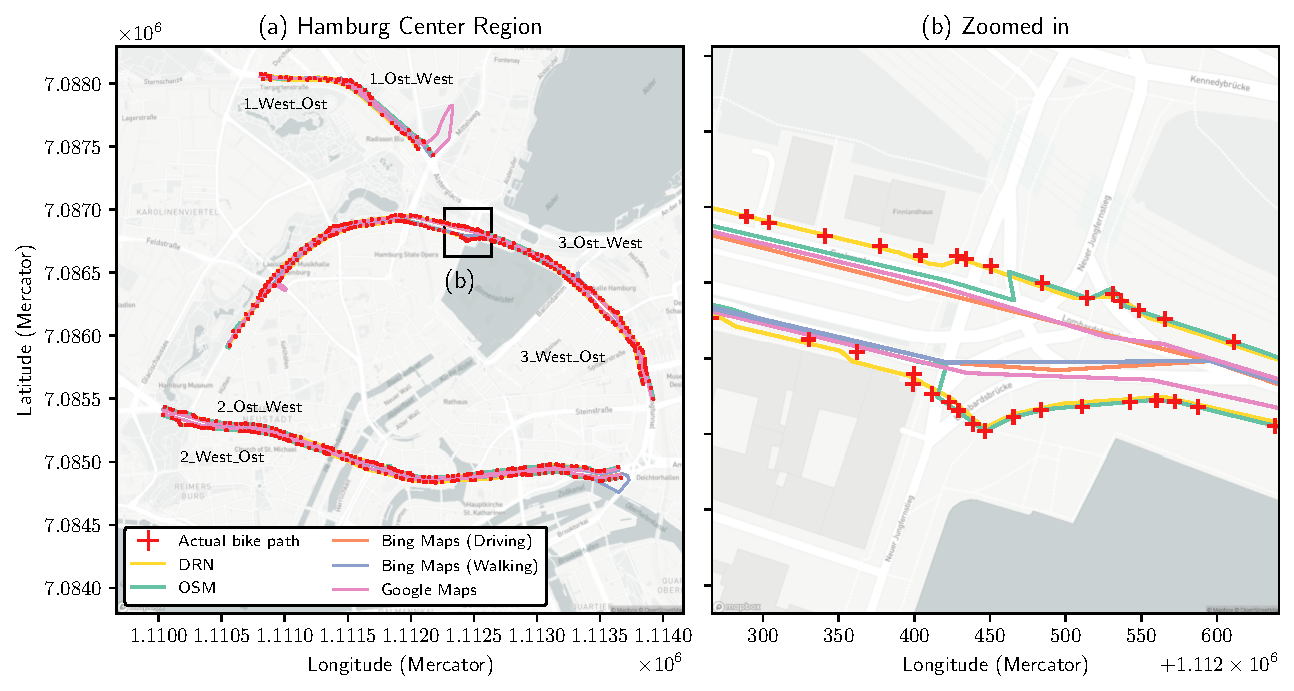
\includegraphics[width=\linewidth]{images/routing-hand-drawn-ground-truth.pdf}
\caption{.}
\label{fig:routing-hand-drawn-ground-truth}
\end{figure}

Six reference tracks were created, containing three pairs of routes running in opposite directions: one from east to west and one from west to east. These reference tracks are depicted in \Cref{fig:routing-hand-drawn-ground-truth} as red cross-marks. Afterward, routes are generated by the map providers and compared for alignment with the reference geometry. Although it would be possible to use corresponding map-matching APIs here, the intention is to emulate user behavior in creating waypoints and check whether the generated route matches the reference geometry. In this experiment, we assume that the user wants to follow the reference geometry as accurately as possible.

One challenge during this process is a curved reference geometry such as \texttt{3\_West\_Ost}, which tends to be shortcutted via a more direct connection between start and endpoints. Thus, assuming that a user wants to follow the reference track, the number of waypoints is gradually increased from 2 to 10 using the same interpolation across all compared providers. In each step, the alignment is measured, ultimately taking the best fit out of all attempts to give each provider multiple chances at generating the most accurate route. In this way, not only the best alignment is measured, but also the tendency to deviate from an intended route even when new waypoints are added, indicating the user's intention.

\begin{table}[t]
\centering
\resizebox{\linewidth}{!}{%
\begin{tabular}{llrrrrrr}
\toprule
\textbf{Routing} & \textbf{Metric} & \rotatebox{0}{\textbf{\texttt{1\_Ost\_West}}} & \rotatebox{0}{\textbf{\texttt{1\_West\_Ost}}} & \rotatebox{0}{\textbf{\texttt{2\_Ost\_West}}} & \rotatebox{0}{\textbf{\texttt{2\_West\_Ost}}} & \rotatebox{0}{\textbf{\texttt{3\_West\_Ost}}} & \rotatebox{0}{\textbf{\texttt{3\_Ost\_West}}} \\
\midrule
DRN & Hausdorff distance (m) & 6.9 & 2.8 & 3.5 & 3.7 & 4.7 & 7.8 \\
 & Mean distance (m) & 2.2 & 1.2 & 1.1 & 1.0 & 1.7 & 1.4 \\
 & \# Waypoints for best fit & 2 & 2 & 3 & 3 & 4 & 3 \\
 & Length difference (m) & -7.6 & -1.7 & -1.7 & -0.7 & 0.8 & 5.1 \\
\hline
OpenStreetMap & Hausdorff distance (m) & 3.5 & 9.1 & 14.4 & 10.6 & 15.2 & 16.0 \\
 & Mean distance (m) & 1.3 & 6.0 & 4.4 & 2.9 & 6.3 & 4.7 \\
 & \# Waypoints for best fit & 8 & 2 & 9 & 7 & 4 & 8 \\
 & Length difference (m) & 1.0 & 5.8 & 147.3 & 11.5 & 67.4 & 26.7 \\
\hline
Bing Maps & Hausdorff distance (m) & 16.3 & 14.7 & 17.8 & 26.9 & 25.9 & 18.1 \\
(Driving) & Mean distance (m) & 9.7 & 9.0 & 10.5 & 11.4 & 10.0 & 8.5 \\
 & \# Waypoints for best fit & 4 & 7 & 2 & 2 & 8 & 8 \\
 & Length difference (m) & -20.8 & 11.1 & -2.1 & -10.0 & -0.9 & -29.9 \\
\hline
Bing Maps & Hausdorff distance (m) & 16.0 & 14.7 & 17.8 & 67.4 & 27.1 & 41.6 \\
(Walking) & Mean distance (m) & 9.6 & 9.0 & 10.9 & 16.8 & 10.1 & 13.4 \\
 & \# Waypoints for best fit & 8 & 7 & 8 & 2 & 3 & 6 \\
 & Length difference (m) & 56.3 & 11.1 & 19.1 & 117.8 & -1.7 & 58.3 \\
\hline
Google Maps & Hausdorff distance (m) & 216.4 & 8.7 & 19.3 & 26.3 & 52.6 & 16.7 \\
 & Mean distance (m) & 66.5 & 6.1 & 10.7 & 10.5 & 11.4 & 7.6 \\
 & \# Waypoints for best fit & 2 & 9 & 3 & 2 & 9 & 3 \\
 & Length difference (m) & 418.9 & 26.0 & -7.2 & -18.7 & 123.6 & -35.5 \\
\bottomrule
\end{tabular}
}
\caption{Measured deviations from actual bike infrastructure.}%
\label{tab:accuracy-comparison}%
\end{table}

The alignment is measured by two metrics: the Hausdorff distance, an established measure to calculate two geometries' shapes, and the mean distance, as calculated through the Vincenty estimator, accurate up to 0.5mm. The Hausdorff distance is calculated through the Shapely\footnote{\url{https://github.com/shapely/shapely}} Python library in the EPSG:32633\footnote{\url{https://epsg.io/32633}} projection that utilizes meters as a distance unit. It is also utilized as a reference to determine the best-fitting route. To additionally measure detours and the overall estimation quality of path length, we also calculate the difference in length, subtracting the length of the reference geometry from the route's length, again using the Vincenty estimator. Here, negative values indicate an underestimation and positive values indicate an overestimation of the actual path length.

As depicted in \Cref{fig:routing-hand-drawn-ground-truth}, four routing providers are compared: our method DRN, OpenStreetMap using a GraphHopper, the Bing Maps routing API\footnote{\url{https://learn.microsoft.com/en-us/bingmaps/rest-services/routes/calculate-a-route}}, and the Google Maps routing API\footnote{\url{https://developers.google.com/maps/documentation/routes/reference/rest/v2/TopLevel/computeRoutes?hl=de}}. For DRN and OpenStreetMap, the GraphHopper routing profile \texttt{bike2} is utilized. For Google Maps, \texttt{travelMode=\allowbreak BICYCLE} is selected. Bing Maps is utilized by the modes \texttt{Driving} and \texttt{Walking} as no bike mode is provided, to determine which option is the best proxy for a bike route.

The best fits are highlighted in \Cref{fig:routing-hand-drawn-ground-truth}. In example (b), it can be seen that the DRN bike route aligns almost perfectly with the hand-drawn reference track. The OpenStreetMap route generated by GraphHopper tends to switch between the bike path and the center of the road -- a behavior seen before in \Cref{ch:matching} with this routing foundation. However, OpenStreetMap is still closer to the bike infrastructure than Google Maps and both Bing Maps routing profiles. In this case, choosing the \texttt{Walking} profile for Bing Maps seems to make no significant difference in whether the footpath is chosen.

\begin{figure}[t]
\centering 
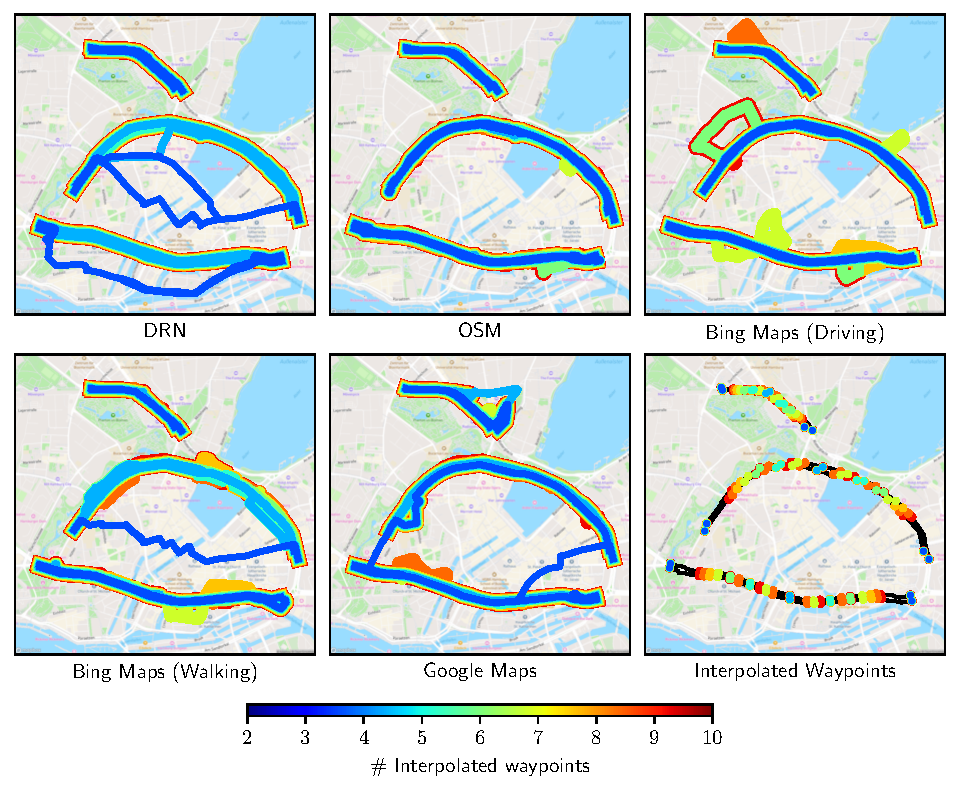
\includegraphics[width=\linewidth]{images/routing-convergence-process.pdf}
\caption{.}
\label{fig:routing-convergence-process}
\end{figure}

Both commercial providers, Bing Maps and Google Maps, seem to produce a less detailed geometry in the given example. Minor bends are not captured. \Cref{tab:accuracy-comparison} shows that the observations from the case study also align with our numerical measurements. As DRN produces no detours in this sample and captures minor road bends that are contained in the reference material as well, its estimated path length aligns closely with the actual path length as represented by our hand-drawn trajectories. Except for \texttt{1\_Ost\_West}, on which OpenStreetMap achieves the best Hausdorff and mean distances, DRN performs substantially better in depicting bike infrastructure than all other routing foundations in the studied examples. Under the remaining routing foundations, OpenStreetMap seems to provide the generally most accurate depiction. Both \texttt{Walking} and \texttt{Driving} routing profiles for Bing Maps produce similar results.

Based on the number of waypoints DRN required to achieve the best fit, it seems to converge more quickly on the desired trajectory compared to the other routing foundations. As shown in \Cref{fig:routing-convergence-process}, only the first one or two routes providing two or three waypoints, respectively, deviate from the intended path in DRN. In one example that is also challenging for other routing foundations, \texttt{3\_West\_Ost}, DRN requires four waypoints to snap to the desired paths.

Overall, OpenStreetMap has a quick convergence on the desired paths in these examples. However, it also seems to be more unstable when additional waypoints are added to the trajectory in some cases and produce visibly unnecessary detours. The same behavior can be seen with the other routing foundations, especially Google Maps, which did not want to converge fully onto the \texttt{1\_Ost\_West} trajectory no matter the number of waypoints, inserting a large detour instead. Bing Maps also inserted visibly unnecessary detours. 

As it is likely that an origin for the observed detours is waypoints that reside on a non-captured path within the routing foundations, these results may look different whenever the waypoints are slightly offset. Thus, the observations w.r.t. unnecessary detours made in this experiment, although generally valid, may not generalize to an overarching assessment of the routing foundations' accuracies. Nonetheless, the experiments, although being limited to six trajectories, already send a clear signal that the developed routing service provides substantially more accurate bike routes. To draw further conclusions, we will conduct further larger-scale analyses in the upcoming sections.

\subsection{Alignment with Traffic Light Geometries}

As discussed in \Cref{ch:matching}, georeferenced intersection topologies provide the foundation for traffic light matching in this work. Each intersection topology contains ingress, connection, and egress lane shapes for each traffic light. Since the traffic light geometries are designed to depict turn shapes at intersections as accurately as possible, they provide another option to evaluate the alignment of the developed routing network with a special focus on intersections. A close alignment is desired to enhance the accuracy of traffic light matching.

As only one or a few traffic lights may match a given bike route at an intersection, we cannot directly compare all traffic light geometries with the routing foundation. As we have seen in \Cref{ch:matching}, many traffic lights are never a good option in the presence of a better alternative aligning closer with the bike path that predicts the cyclist's trajectory. Thus, we first calculate bike routes with DRN and manually select fitting traffic light geometries. Afterward, we can compare the traffic light geometries to the corresponding route to measure their alignment. 

\begin{figure}[htbp]
\centering 
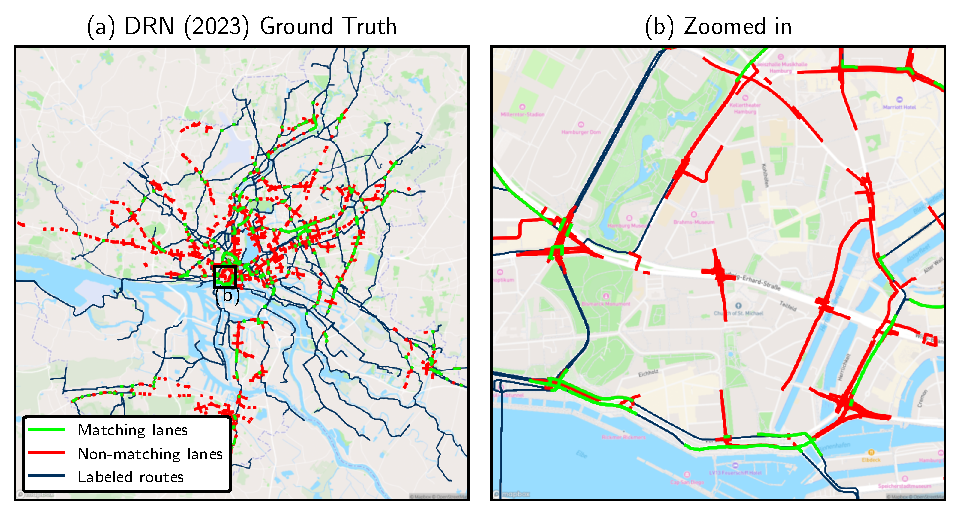
\includegraphics[width=\linewidth]{images/matching-ground-truth-drn.pdf}
\caption{.}
\label{fig:matching-ground-truth-drn}
\end{figure}

The DRN traffic light matching ground truth was developed according to the same procedures explained detailedly in \Cref{ch:matching}. The resulting mapping between generated DRN routes and traffic light geometries is depicted in \Cref{fig:matching-ground-truth-drn}. It contains 49 routes randomly distributed in Hamburg, for which 738 traffic light geometries have been selected in total to match the route geometry. These 738 selections can be mapped to 535 distinct traffic lights that were assigned to at least one route. 78.5\% (420) of traf are assigned to only one route. 

- 2. Wir schauen uns an, ob die passenden Ampelgeometrien tendenziell näher an der generierten Route liegen, im Vergleich zu OpenStreetMap für das eine Ground Truth schon in \Cref{ch:matching} erstellt wurde

\begin{figure}[htbp]
\centering 
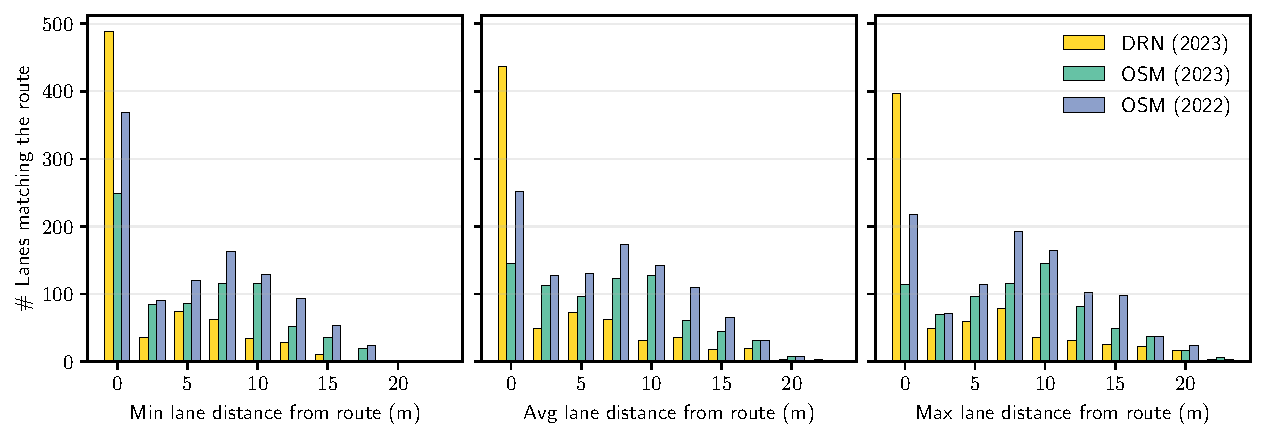
\includegraphics[width=\linewidth]{images/routing-lane-alignment.pdf}
\caption{.}
\label{fig:}
\end{figure}

\begin{figure}[htbp]
\centering 
\begin{tabular}{ccc}
\footnotesize{(b) Samples from OpenStreetMap Ground Truth (2023)} & \footnotesize{(b) Samples from DRN Ground Truth (2023)}  \\
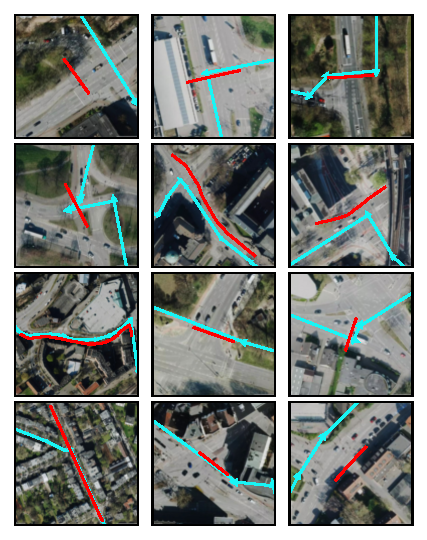
\includegraphics[width=0.46\linewidth]{images/routing-lane-alignment-examples-osm.pdf} & 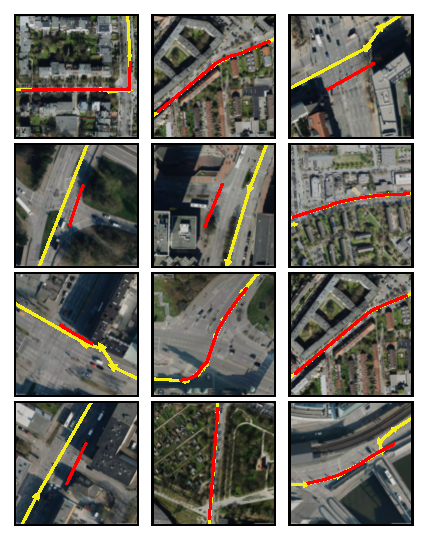
\includegraphics[width=0.46\linewidth]{images/routing-lane-alignment-examples-drn.pdf} \\
\end{tabular}
\caption{.}
\label{fig:}
\end{figure}

- 3. Wir trainieren das Traffic Light Matching modell erneut auf der neuen DRN Ground Truth und schauen, ob dieses die Ampeln auf DRN akkurater matchen kann

\begin{table}[h]
\caption{Retrained model thresholds on the new routing.}
\begin{tabular}{@{}llllllllll@{}}
\toprule
  \textbf{Ground Truth} & $t_{dist}$ & $t_{bear}$ & $t_{bear\_sum}$ & $t_{inv}$ & $t_{len}$ & $t_{len\_sum}$ & $t_{road\_side}$ &  $t_{perfect\_m.}$ & $t_{overlap}$ \\
  \midrule
  OSM (2022) & 20m & 33° & 79\% & False & 0.99 & 93\% & 59m & 50m & 43\% \\
  OSM (2023) & 19m & 50° & 78\% & False & 0.96 & 77\% & 95m & 46m & 5\% \\
  DRN (2023) & 17m & 27° & 73\% & False & 0.81 & 61\% & 48m & 43m & 59\% \\
\bottomrule
\end{tabular}
\label{tab:hyperparameter-tuning-results-drn}
\end{table}

\begin{table}[h]
\caption{.}
\begin{tabular}{@{}lllllllll@{}}
\toprule
  \textbf{Model} & \textbf{Benchmark} & \textbf{Trained on} & \textbf{TP} & \textbf{FP} & \textbf{FN} & \textbf{Precision} & \textbf{Recall} & \textbf{F1} \\
  \midrule
  Algorithmic & OSM 2022 & OSM 2022 & 920 & 207 & 123 & 82\% & 88\% & 84.8\% \\
  Algorithmic & OSM 2022 & OSM 2023 & 908 & 221 & 135 & 80\% & 87\% & 83.6\% \\
  ML          & OSM 2022 & OSM 2022 & 936 & 57 & 107 & 94\% & 90\% & 91.9\% \\
  \midrule
  Algorithmic & OSM 2023 & OSM 2022 & 615 & 159 & 143 & 79\% & 81\% & 80.3\% \\
  Algorithmic & OSM 2023 & OSM 2023 & 637 & 136 & 121 & 82\% & 84\% & 83.2\% \\
  ML          & OSM 2023 & OSM 2022 & 614 & 52 & 144 & 92\% & 81\% & 86.2\% \\
  \midrule
  Algorithmic & DRN 2023 & DRN 2023 & 655 & 95 & 83 & 87\% & 89\% & 88.0\% \\
  ML          & DRN 2023 & DRN 2023 & 676 & 24 & 62 & 97\% & 92\% & 94.0\% \\
\bottomrule
\end{tabular}
\label{tab:model-scores-drn}
\end{table}

- 4. Wir schauen uns an, in welcher Konstellation DRN-Routen häufig über Ampelgeometrien verlaufen - also ob die geometrien gleicher verlaufen als mit OpenStreetMap.

\begin{figure}[htbp]
\centering 
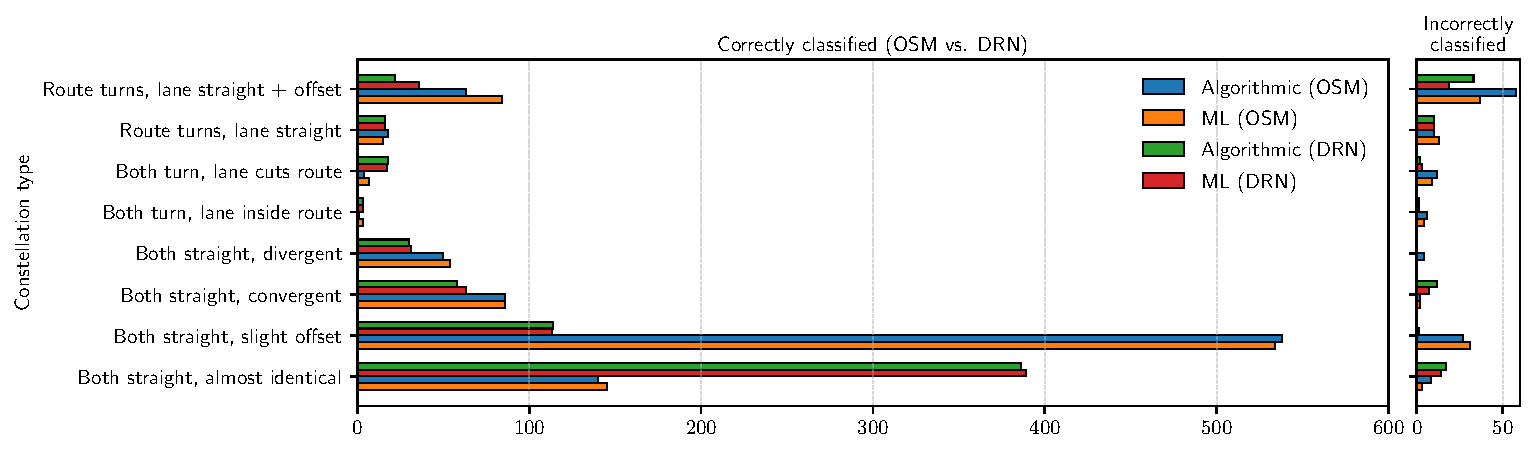
\includegraphics[width=\linewidth]{images/matching-constellations-osm-vs-drn.pdf}
\caption{.}
\label{fig:}
\end{figure}

- 5. Abschließend schauen wir uns nochmal an, wie viele Routenfehler an den Kreuzungen vorkommen, im Vergleich zwischen DRN und OSM. In einer detailliertern Analyse entlang ganzer Routen (nicht nur auf die Kreuzung bezogen) schauen wir uns nochmal genauere Routenfehlertypen an, und wie häufig diese im Vergleich vorkommen.

\begin{figure}[htbp]
\centering 
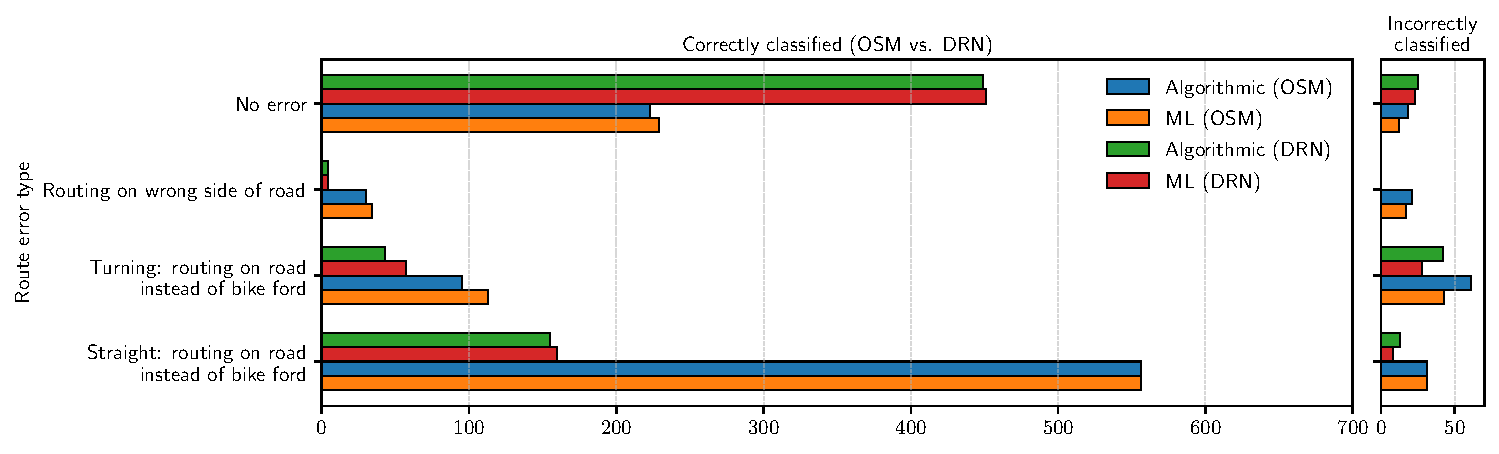
\includegraphics[width=\linewidth]{images/matching-route-errors-osm-vs-drn.pdf}
\caption{.}
\label{fig:}
\end{figure}

\begin{table}[htbp]
\centering
\begin{tabular}{lrr}
\hline
\textbf{Observed Error Cases} & DRN & OpenStreetMap \\ \hline
Continuous routing on the road & 0 & 10 \\
Routing through buildings or stairs & 0 & 2 \\
Intersection crossing using car lanes & 0 & 8 \\
Use of sidewalks on incorrect road side & 1 & 4 \\
Missing permission for one-way streets & 0 & 1 \\
Routing through other impassable obstacles & 0 & 2 \\
Failure to consider turning restrictions & 0 & 1 \\
Skipping or crossing additional signals & 1 & 3 \\
Generally problematic road crossings & 1 & 4 \\
\hline
\end{tabular}
\caption{Observed error cases among arbitrary sample of 72 routes.}%
\label{tab:accuracy-comparison}%
\end{table}

\subsection{Alignment with User Trajectories}

\begin{figure}[htbp]
\centering 
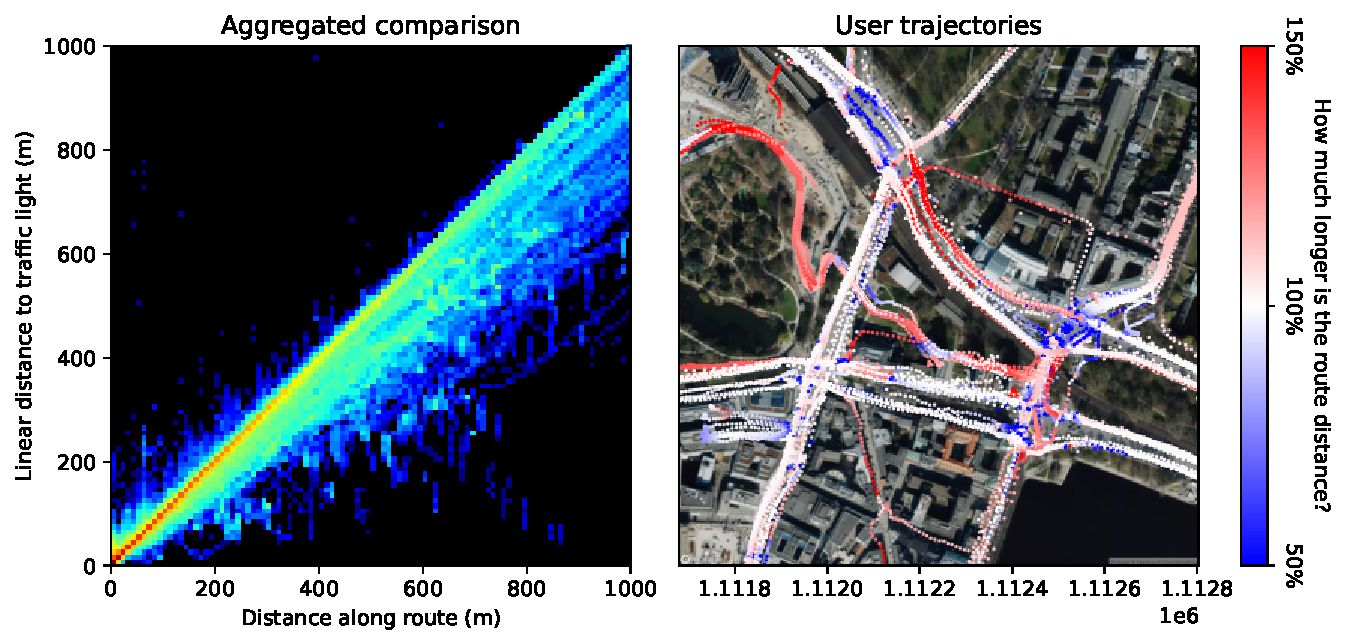
\includegraphics[width=\linewidth]{images/routing-distance-analysis.pdf}
\caption{.}
\label{fig:}
\end{figure}


\begin{figure}[htbp]
\centering 
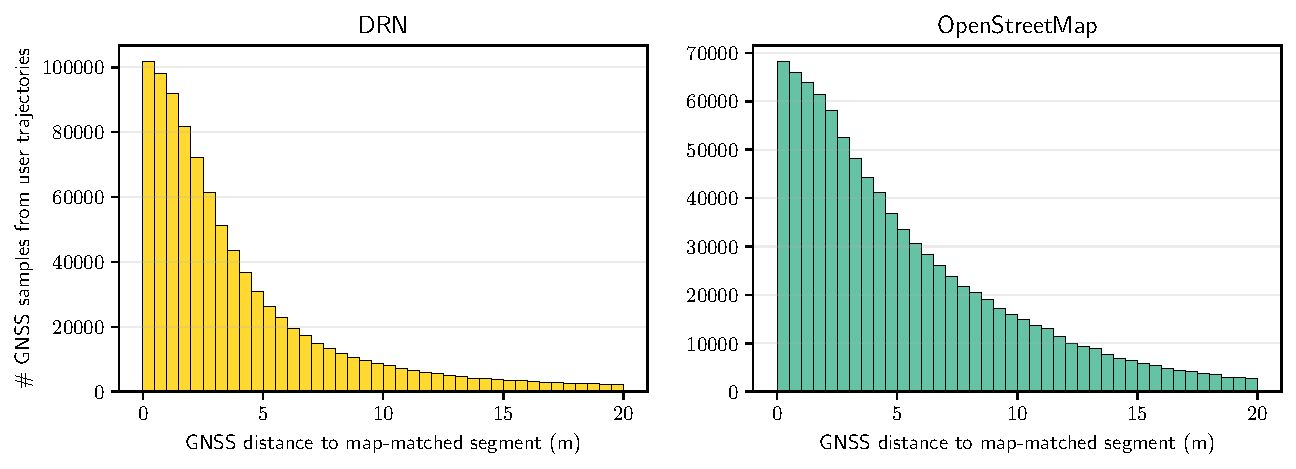
\includegraphics[width=\linewidth]{images/routing-gnss-mapmatching-distribution.pdf}
\caption{.}
\label{fig:}
\end{figure}

\begin{figure}[htbp]
\centering 
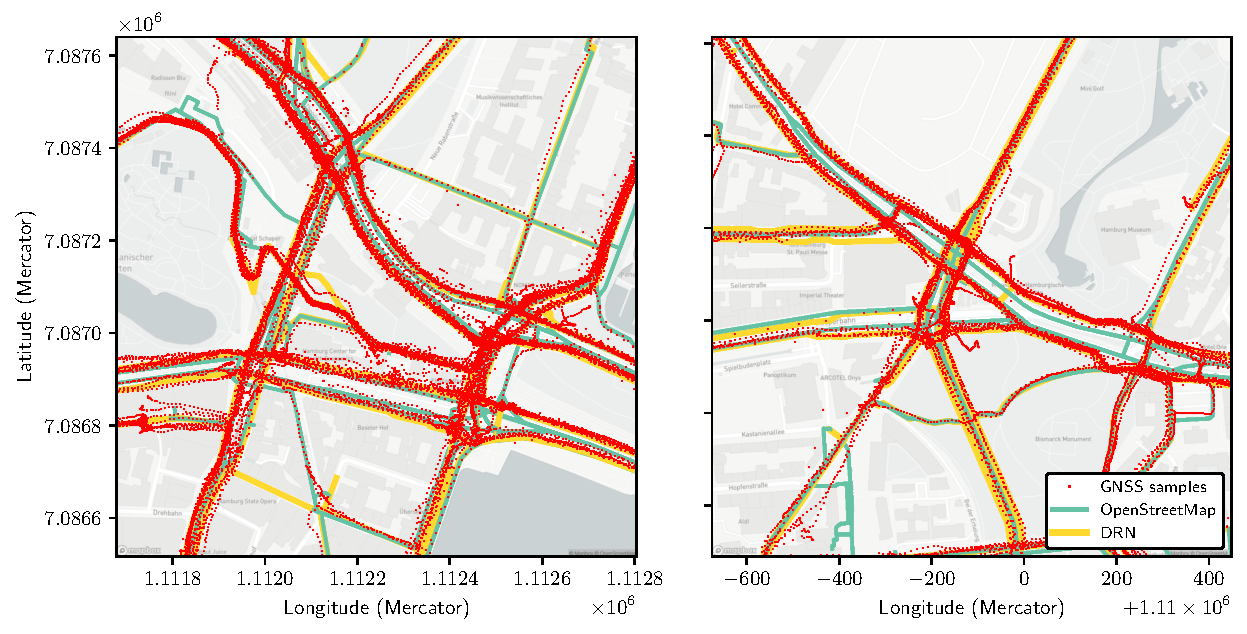
\includegraphics[width=\linewidth]{images/routing-mapmatching-distance.pdf}
\caption{.}
\label{fig:}
\end{figure}

\begin{figure}[htbp]
\centering 
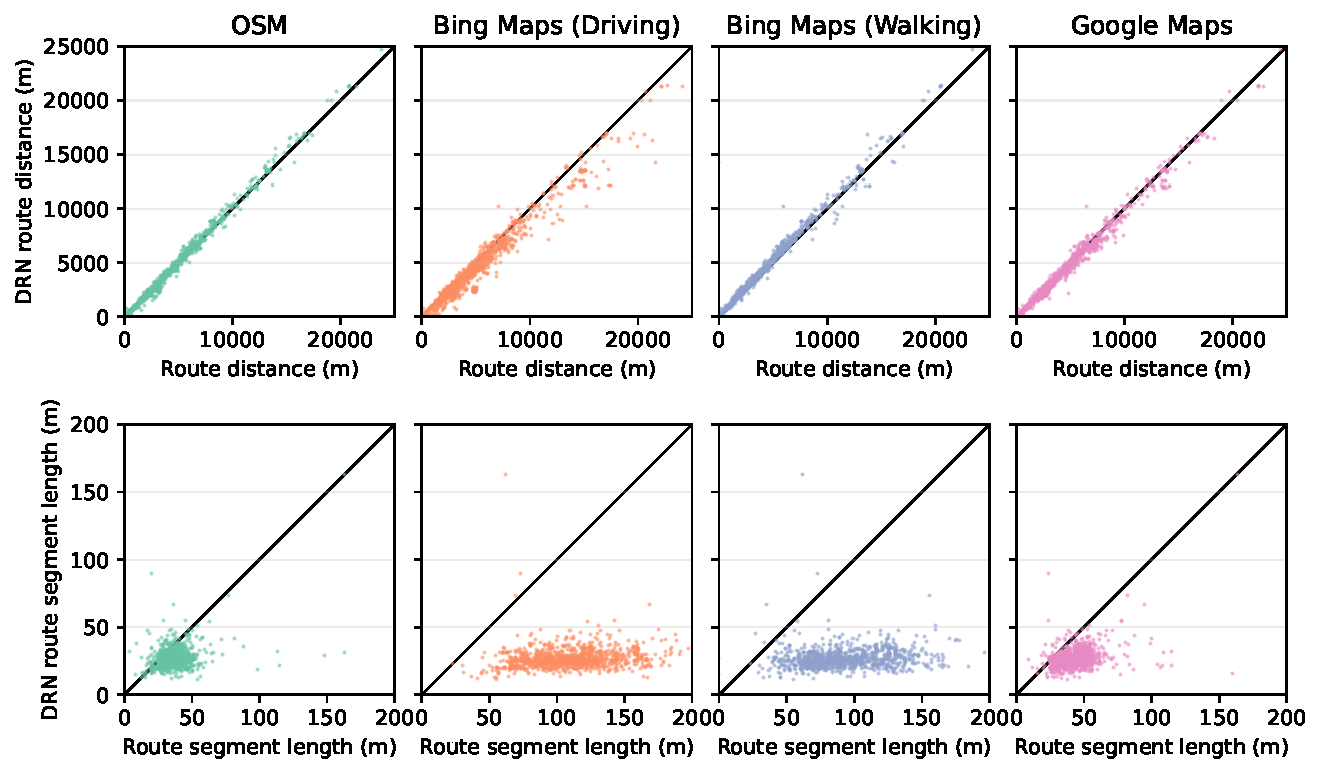
\includegraphics[width=\linewidth]{images/routing-distance-comparison.pdf}
\caption{.}
\label{fig:}
\end{figure}

\section{Conclusions}